\documentclass[11pt,a4paper,openany]{book}

\usepackage[utf8]{inputenc}
\usepackage[T1]{fontenc}
\usepackage{amsmath,amssymb,amsfonts,amsthm}
\usepackage{geometry}
\geometry{a4paper, left=2.2cm, right=2.2cm, top=2.5cm, bottom=2.5cm}

\newtheorem{theorem}{Theorem}[chapter]
\newtheorem{proposition}[theorem]{Proposition}
\newtheorem{lemma}[theorem]{Lemma}
\theoremstyle{definition}
\newtheorem{definition}[theorem]{Definition}

\usepackage{booktabs}
\usepackage{array}
\usepackage{longtable}
\usepackage{pdfpages}
\usepackage{csquotes}
\MakeOuterQuote{"}

\usepackage[table]{xcolor}
\definecolor{mosaicblue}{RGB}{74, 128, 196}
\definecolor{mosaicpink}{RGB}{224, 102, 102}
\definecolor{faintrule}{gray}{0.78}

\usepackage{tikz}
\usetikzlibrary{shapes.geometric, calc}

\usepackage[pdfusetitle, hidelinks, colorlinks=true, linkcolor=blue!70!black, citecolor=blue!70!black, urlcolor=blue!70!black]{hyperref}

\title{\textbf{An Atlas of Composition Mosaics}\\[0.4em]
\Large The Complete Dihedral Universe from $\mathbb{Z}_1$ to $\mathbb{Z}_9$}
\author{Gemma Knee \and Antigra Vitti}
\date{November 2026}

\begin{document}

\frontmatter
\maketitle

\chapter*{Preface}
\addcontentsline{toc}{chapter}{Preface}
\markboth{Preface}{Preface}

This volume presents the complete visual classification, combinatorial taxonomy, and machine-readable relational inventory of composition mosaics across the circular rings $\mathbb{Z}_1$ through $\mathbb{Z}_9$.

As the third monograph in our coffee-table trilogy on the combinatorial geometry of circular lattices---standing alongside \emph{The Polygonal Burnsidean: An Atlas of Inscribed Polygons from $\mathbb{Z}_1$ to $\mathbb{Z}_{16}$} and \emph{Hexadecality: The Atlas of Hexadecagonal Compositions}---this atlas unifies the full progression of cyclic lattices from the elementary monad to the rich enneagonal universe:
\begin{itemize}
    \item Across the first nine rings $\mathbb{Z}_1$ through $\mathbb{Z}_9$, the combinatorial universe generates exactly $26{,}442$ set partitions, governed by the initial segment of the Bell numbers $B_1 = 1, B_2 = 2, B_3 = 5, B_4 = 15, B_5 = 52, B_6 = 203, B_7 = 877, B_8 = 4{,}140$, and $B_9 = 21{,}147$.
    \item Under the physical symmetries of the respective dihedral groups $D_n$, these $26{,}442$ partitions collapse into exactly $\mathbf{1{,}859}$ non-equivalent dihedral composition mosaics, realising the initial terms of sequence OEIS A084708:
    \begin{equation*}
    1, \; 2, \; 3, \; 7, \; 12, \; 37, \; 93, \; 354, \; 1{,}350 \quad \implies \quad \sum_{n=1}^9 M_n = 1{,}859
    \end{equation*}
    \item The nine lattices capture the full structural spectrum of cyclic geometry: the trivial monad $\mathbb{Z}_1$; the reflexive dyad $\mathbb{Z}_2$; the odd prime rings $\mathbb{Z}_3, \mathbb{Z}_5, \mathbb{Z}_7$; the composite square lattice $\mathbb{Z}_4$; the composite hexagonal lattice $\mathbb{Z}_6$ where scalene triangles and chiral enantiomorphic blocks first emerge into the geometric universe; the cubic power-of-two lattice $\mathbb{Z}_8$, which hosts the unique cyclic Skolem difference sequence of order $4$; and the nonagonal lattice $\mathbb{Z}_9$, whose ternary modular geometry exhibits rich threefold rotational symmetries and modular prime-power factorisations.
    \item Through the two-vertex domino inflation functor, the 8-vertex Skolem partition acts as the seed for higher-order affine macro-orbits on the 16-cycle $\mathbb{Z}_{16}$, creating an explicit mathematical bridge connecting all three volumes of the trilogy.
\end{itemize}

\section*{Cartographic Conventions and Visual Aesthetics}

Each mosaic in this atlas is presented in pure geometric form. The partition blocks appear as shaded convex inscribed polygons, metric chords, and vertex pips within the circular frame of the regular $n$-gon, unencumbered by peripheral coordinate clutter:
\begin{itemize}
    \item \textbf{Achiral Blocks (Blue)}: Inscribed polygons possessing an internal axis of bilateral reflection symmetry across the cyclic lattice.
    \item \textbf{Chiral Blocks (Pink)}: Scalene polygons that lack reflectional symmetry, existing as one half of an enantiomorphic pair.
\end{itemize}

The complete visual catalogue in Chapter~\ref{chap:visual-atlas} displays all $1{,}859$ configurations arranged in a strict taxonomic sequence across 33 high-density vector plates. All accompanying analytical invariants---dihedral orbit sizes $|\mathcal{O}|$, stabiliser subgroups, Fa\`a di Bruno partition multiplicities, chord dispersion energies, polygon profiles, and relational manifests linking directly into \emph{The Polygonal Burnsidean}---are systematically catalogued in Chapter~\ref{chap:canonical-taxonomy} and in the companion machine-readable open datasets.

\bigskip
\begin{flushright}
\textbf{Gemma Knee} \qquad \textbf{Antigra Vitti} \\
\emph{Newcastle upon Tyne} \\
\emph{November 2026}
\end{flushright}


\tableofcontents
\clearpage
\listoftables

\mainmatter

\chapter{Lattice Geometry and Combinatorial Invariants}
\label{chap:lattice-architecture}

\section{Circular Lattices and Dihedral Symmetries}

Let $\mathbb{Z}_n = \{0, 1, \dots, n-1\}$ denote the cyclic ring of integers modulo $n$, geometrically embedded as the vertices of a regular $n$-gon inscribed in the unit circle and oriented clockwise with vertex $0$ positioned at the zenith. 

The physical isometries of the polygon constitute the dihedral group $D_n$. Geometrically, $D_n$ is generated by two reflections $\tau$ and $\tau' = \tau \rho$ whose reflection axes intersect at angle $\pi / n$. In the classical reflection (Coxeter) presentation, the group is given by:
\begin{equation}
D_n = \langle \rho, \tau \mid \rho^n = \tau^2 = (\tau \rho)^2 = 1 \rangle
\end{equation}
where $\rho = \tau \tau'$ is the clockwise unit rotation $x \mapsto x + 1 \pmod n$ and $\tau$ is the vertical chord reflection $x \mapsto -x \equiv n - x \pmod n$. In academic literature, the involution relation $(\tau \rho)^2 = 1$ is frequently rewritten as the conjugation relation:
\begin{equation}
\tau \rho \tau = \rho^{-1}
\end{equation}
emphasising the semidirect product decomposition $D_n \cong \mathbb{Z}_n \rtimes \mathbb{Z}_2$, in which the reflection $\tau \in \mathbb{Z}_2$ acts on the normal cyclic subgroup $\langle \rho \rangle \cong \mathbb{Z}_n$ by group inversion ($x \mapsto -x$). For the degenerate small rings, the isometry groups coincide with the physical symmetries:
\begin{equation}
D_1 = \{1\} \; (|D_1| = 1), \qquad D_2 = \langle \rho \mid \rho^2 = 1 \rangle \cong C_2 \; (|D_2| = 2)
\end{equation}
where on two vertices the single reflection $x \mapsto 1 - x \pmod 2$ acts identically to the transposition rotation $\rho$. For any $n \ge 1$, the reflections in $D_n$ are precisely the involutions $x \mapsto b - x \pmod n$ for $b \in \mathbb{Z}_n$.

A \textbf{composition mosaic} $\mathcal{M}$ on $\mathbb{Z}_n$ is a set partition of the $n$ vertices into $s$ non-empty, pairwise disjoint blocks:
\begin{equation}
\mathcal{M} = \{B_1, B_2, \dots, B_s\}, \quad \bigcup_{j=1}^s B_j = \mathbb{Z}_n, \quad B_i \cap B_j = \emptyset \; (i \neq j)
\end{equation}
Each constituent block $B_j \subset \mathbb{Z}_n$ of cardinality $d_j = |B_j| \ge 1$ forms an inscribed polygon in the lattice:
\begin{itemize}
    \item A \textbf{unigon} ($d_j = 1$), visualised as a central circular pip on vertex $v \in \mathbb{Z}_n$.
    \item A \textbf{digon} ($d_j = 2$), visualised as a straight metric chord connecting the vertex pair.
    \item An \textbf{inscribed polygon} ($d_j \ge 3$), visualised as a shaded convex polygonal tile bounded by circular perimeter chords.
\end{itemize}

\section{The Graded Stratification of Set Partitions}

Across the full combinatorial universe, the total number of set partitions of an $n$-element set is given by the $n$-th Bell number $B_n$:
\begin{equation}
B_n = \sum_{s=1}^n \genfrac{\{}{\}}{0pt}{}{n}{s}
\end{equation}
where $\genfrac{\{}{\}}{0pt}{}{n}{s}$ denotes the Stirling numbers of the second kind, enumerating set partitions into exactly $s$ blocks. 

The space of partitions further stratifies according to the unordered multiset of block sizes, termed the \textbf{partition shape} $\lambda = (\lambda_1, \dots, \lambda_s) \vdash n$, where $\lambda_1 \ge \lambda_2 \ge \dots \ge \lambda_s \ge 1$ and $\sum_{j=1}^s \lambda_j = n$. For each shape $\lambda \vdash n$, the exact number of set partitions is governed by the Fa\`a di Bruno multinomial formula:
\begin{equation}
p_\lambda = \frac{n!}{\prod_{i=1}^n (i!)^{c_i} \, c_i!}
\end{equation}
where $c_i = c_i(\lambda)$ is the multiplicity of parts of size $i$ in $\lambda$.

Across the first nine rings $\mathbb{Z}_1$ through $\mathbb{Z}_9$, the Bell numbers grow rapidly:
\begin{gather*}
B_1 = 1, \quad B_2 = 2, \quad B_3 = 5, \quad B_4 = 15, \quad B_5 = 52 \\
B_6 = 203, \quad B_7 = 877, \quad B_8 = 4{,}140, \quad B_9 = 21{,}147
\end{gather*}
yielding a core combinatorial universe of $26{,}442$ set partitions across $96$ integer partition shapes. Extending this progression through $\mathbb{Z}_{16}$ reveals the full exponential escalation of the partition continuum, reaching $B_{16} = 10{,}480{,}142{,}147$ and encompassing a cumulative universe of $12{,}086{,}679{,}035$ set partitions across $914$ partition shapes.

\section{The Dihedral Orbit Inventory and Burnsidean Enumeration}

The dihedral group $D_n$ acts on the space of set partitions $\mathcal{P}(\mathbb{Z}_n)$ by permuting the underlying coordinates:
\begin{equation}
g \cdot \{B_1, \dots, B_s\} = \{g(B_1), \dots, g(B_s)\} \quad (g \in D_n)
\end{equation}
Because the group action is an isometry, it preserves the part count $s$, the individual block cardinalities $|B_j|$, and the partition shape $\lambda \vdash n$. The set partitions of shape $\lambda$ decompose into disjoint $D_n$-orbits:
\begin{equation}
\mathcal{O}(\mathcal{M}) = \{g \cdot \mathcal{M} \mid g \in D_n\}
\end{equation}

By the Orbit-Stabiliser Theorem, the length of any orbit $|\mathcal{O}| = k$ must divide the group order $|D_n|$. The stabiliser subgroup $\operatorname{Stab}_{D_n}(\mathcal{M})$ has order $|D_n| / k$.

Summing the orbit multiplicities $a_{k,\lambda}$ yields the graded bivariate orbit polynomial $P_n(\mathbf{z}, \omega)$:
\begin{equation}
P_n(\mathbf{z}, \omega) = \sum_{\lambda \vdash n} Q_\lambda(\omega) \mathbf{z}^\lambda = \sum_{\lambda \vdash n} \left( \sum_{k \mid |D_n|} a_{k,\lambda} \omega^k \right) \mathbf{z}^\lambda
\end{equation}
Evaluating this polynomial at $\omega = 1$ recovers the total count $M_n$ of non-equivalent dihedral composition mosaics on $\mathbb{Z}_n$. Table~\ref{tab:census-z1-z16} presents the consolidated inventory across the sixteen rings $\mathbb{Z}_1$ through $\mathbb{Z}_{16}$, recovering the initial sixteen terms of OEIS sequence A084708 and establishing the grand total of $\mathbf{382{,}030{,}946}$ non-equivalent dihedral composition mosaics (of which the initial nine rings comprise the $1{,}859$ visually catalogued mosaics of the core atlas).

% Consolidated Dihedral Mosaic Census from Z1 to Z16
\begin{table}[htbp]
\centering
\small
\setlength{\tabcolsep}{4.5pt}
\caption{\label{tab:census-z1-z16}\label{tab:census-z1-z8}Consolidated Dihedral Mosaic Census from $\mathbb{Z}_1$ to $\mathbb{Z}_{16}$ (OEIS A084708)}
\begin{tabular}{c r r r r l}
\toprule
Ring $\mathbb{Z}_n$ & $|D_n|$ & Partitions $B_n$ & Shapes & Dihedral Mosaics & Orbit Size Decomposition $\sum a_k \omega^k$ \\
\midrule
$\mathbb{Z}_1$ & 1 & 1 & 1 & \textbf{1} & $1\omega^{1}$ \\
$\mathbb{Z}_2$ & 2 & 2 & 2 & \textbf{2} & $2\omega^{1}$ \\
$\mathbb{Z}_3$ & 6 & 5 & 3 & \textbf{3} & $2\omega^{1} + 1\omega^{3}$ \\
$\mathbb{Z}_4$ & 8 & 15 & 5 & \textbf{7} & $3\omega^{1} + 2\omega^{2} + 2\omega^{4}$ \\
$\mathbb{Z}_5$ & 10 & 52 & 7 & \textbf{12} & $2\omega^{1} + 10\omega^{5}$ \\
$\mathbb{Z}_6$ & 12 & 203 & 11 & \textbf{37} & \begin{tabular}[t]{@{}l@{}} $4\omega^{1} + 2\omega^{2} + 9\omega^{3} + {}$ \\ $\quad 16\omega^{6} + 6\omega^{12}$ \end{tabular} \\
$\mathbb{Z}_7$ & 14 & 877 & 15 & \textbf{93} & $2\omega^{1} + 57\omega^{7} + 34\omega^{14}$ \\
$\mathbb{Z}_8$ & 16 & 4{,}140 & 22 & \textbf{354} & \begin{tabular}[t]{@{}l@{}} $4\omega^{1} + 6\omega^{2} + 27\omega^{4} + {}$ \\ $\quad 132\omega^{8} + 185\omega^{16}$ \end{tabular} \\
$\mathbb{Z}_9$ & 18 & 21{,}147 & 30 & \textbf{1{,}350} & \begin{tabular}[t]{@{}l@{}} $3\omega^{1} + 13\omega^{3} + 323\omega^{9} + {}$ \\ $\quad 1{,}011\omega^{18}$ \end{tabular} \\
$\mathbb{Z}_{10}$ & 20 & 115{,}975 & 42 & \textbf{6{,}351} & \begin{tabular}[t]{@{}l@{}} $4\omega^{1} + 3\omega^{2} + 103\omega^{5} + {}$ \\ $\quad 937\omega^{10} + 5{,}304\omega^{20}$ \end{tabular} \\
$\mathbb{Z}_{11}$ & 22 & 678{,}570 & 56 & \textbf{31{,}950} & \begin{tabular}[t]{@{}l@{}} $2\omega^{1} + 2{,}208\omega^{11} + {}$ \\ $\quad 29{,}740\omega^{22}$ \end{tabular} \\
$\mathbb{Z}_{12}$ & 24 & 4{,}213{,}597 & 77 & \textbf{179{,}307} & \begin{tabular}[t]{@{}l@{}} $6\omega^{1} + 11\omega^{2} + 31\omega^{3} + 38\omega^{4} + {}$ \\ $\quad 288\omega^{6} + 11\omega^{8} + {}$ \\ $\quad 6{,}885\omega^{12} + 172{,}037\omega^{24}$ \end{tabular} \\
$\mathbb{Z}_{13}$ & 26 & 27{,}644{,}437 & 101 & \textbf{1{,}071{,}265} & \begin{tabular}[t]{@{}l@{}} $2\omega^{1} + 16{,}031\omega^{13} + {}$ \\ $\quad 1{,}055{,}232\omega^{26}$ \end{tabular} \\
$\mathbb{Z}_{14}$ & 28 & 190{,}899{,}322 & 135 & \textbf{6{,}845{,}581} & \begin{tabular}[t]{@{}l@{}} $4\omega^{1} + 4\omega^{2} + 1{,}042\omega^{7} + {}$ \\ $\quad 53{,}918\omega^{14} + 6{,}790{,}613\omega^{28}$ \end{tabular} \\
$\mathbb{Z}_{15}$ & 30 & 1{,}382{,}958{,}545 & 176 & \textbf{46{,}162{,}583} & \begin{tabular}[t]{@{}l@{}} $4\omega^{1} + 18\omega^{3} + 162\omega^{5} + 2\omega^{6} + {}$ \\ $\quad 118\omega^{10} + 127{,}459\omega^{15} + {}$ \\ $\quad 46{,}034{,}820\omega^{30}$ \end{tabular} \\
$\mathbb{Z}_{16}$ & 32 & 10{,}480{,}142{,}147 & 231 & \textbf{327{,}731{,}950} & \begin{tabular}[t]{@{}l@{}} $5\omega^{1} + 13\omega^{2} + 121\omega^{4} + 3{,}422\omega^{8} + {}$ \\ $\quad 449{,}637\omega^{16} + 327{,}278{,}752\omega^{32}$ \end{tabular} \\
\bottomrule
\end{tabular}
\end{table}


\section{The Bilateral Symmetry Classification}

Every individual block $B \subset \mathbb{Z}_n$ within a mosaic possesses an internal circular stride composition $(s_1, \dots, s_d)$ satisfying $\sum_{i=1}^d s_i = n$. A block is defined as \textbf{bilaterally symmetric} (or achiral) if it is invariant under at least one reflection $x \mapsto b - x \pmod n$ of the circular lattice. 

Under this classification:
\begin{itemize}
    \item \textbf{Achiral Blocks (Blue)}: Inscribed polygons possessing an internal reflection axis. On any lattice $\mathbb{Z}_n$, every unigon ($d=1$), every digon chord ($d=2$), and every regular or isosceles polygon is strictly achiral.
    \item \textbf{Chiral Blocks (Pink)}: Scalene polygons whose circular stride sequence is not invariant under cyclic reversal.
\end{itemize}

\begin{theorem}[Emergence of Block Chirality]
On the circular lattices $\mathbb{Z}_n$, all constituent blocks of all set partitions are strictly achiral for $n \le 5$. Chiral blocks emerge if and only if $n \ge 6$ and block cardinality $d \ge 3$. The minimal chiral block is the scalene triangle of circular strides $(1, 2, 3)$ on the hexagonal lattice $\mathbb{Z}_6$.
\end{theorem}

\begin{proof}
For block size $d \in \{1, 2\}$, any unigon is trivially self-symmetric, and any digon $\{u, v\}$ is invariant under the reflection through the perpendicular bisector of the chord $u \leftrightarrow v$, which is a valid lattice reflection for every $n$. 

For $d = 3$, an inscribed triangle with stride composition $(s_1, s_2, s_3)$ is chiral if and only if the strides are pairwise distinct (scalene). The minimal sum of three distinct positive integers is $1 + 2 + 3 = 6$. Hence no chiral triangle can exist for $n < 6$. For $n = 6$, the unique integer partition into three distinct parts is $1 + 2 + 3 = 6$, realised by the block $\{0, 1, 3\}$ with strides $(1, 2, 3)$. Under reflection $x \mapsto b - x \pmod 6$, the stride sequence reverses to $(3, 2, 1) \equiv (1, 3, 2) \not\equiv (1, 2, 3)$ under cyclic shifts. Hence $\{0, 1, 3\}$ possesses no internal reflection symmetry and is chiral.
\end{proof}

A mosaic $\mathcal{M}$ is characterised by its \textbf{chirality signature}, recording the binary achiral/chiral character of its sorted constituent blocks (e.g. $[ssss]$ for an all-symmetric mosaic, $[sscc]$ for a mosaic containing two symmetric and two chiral blocks). In the visual atlas, chiral blocks appear in distinctive rose-pink shading, highlighting the subtle symmetry-breaking phenomena that first emerge on $\mathbb{Z}_6$.

\section{The Singleton Shattering Duality}

A foundational structural property uniting all cyclic lattices is the \textbf{Singleton Shattering Duality} (in the spirit of Joyal's combinatorial species and Kerber's permutation representations). For any partition shape $\lambda = (b_1, \dots, b_{s-1}, a) \vdash n$ possessing a distinguished block of size $a \ge 2$, shattering this block into $a$ individual singleton vertices ($a \to 1^a$) forms an equivariant bijection between point stabilisers.

Consequently, the orbit polynomial is identically preserved under singleton replacement:
\begin{equation}
Q_{(b_1, \dots, b_{s-1}, a)}(\omega) \equiv Q_{(b_1, \dots, b_{s-1}, 1^a)}(\omega)
\end{equation}

In particular, for any two-block partition shape $n = a + b$ with distinct block cardinalities $a \ne b$, complementation on the Boolean lattice of subsets induces a \textbf{tripartite shattering triad}:
\begin{equation}
z_a z_b \;\longleftrightarrow\; z_a z_1^b \;\longleftrightarrow\; z_b z_1^a
\end{equation}
Because any lattice isometry $g \in D_n$ fixes a block $A$ setwise if and only if it fixes its complement $B = A^c$, and because $a \ne b$ prevents $g$ from interchanging $A$ and $B$, the stabiliser subgroups satisfy:
\begin{equation}
\operatorname{Stab}_{D_n}(\{A, B\}) = \operatorname{Stab}_{D_n}(A) = \operatorname{Stab}_{D_n}(B) = \operatorname{Stab}_{D_n}(\{A\} \cup \{\{v\} \mid v \in B\})
\end{equation}
Hence all three partition shapes share identical orbit polynomials $Q(\omega)$ across all cyclic lattices:
\begin{align}
\text{On } \mathbb{Z}_4\colon \quad z_4 &\longleftrightarrow z_1^4 && (1\omega^1) \\
\text{On } \mathbb{Z}_5\colon \quad z_5 &\longleftrightarrow z_1^5 && (1\omega^1) \\
\text{On } \mathbb{Z}_6\colon \quad z_6 &\longleftrightarrow z_1^6 && (1\omega^1) \\
z_2 z_4 &\longleftrightarrow z_2 z_1^4 \longleftrightarrow z_4 z_1^2 && (1\omega^3 + 2\omega^6) \\
\text{On } \mathbb{Z}_7\colon \quad z_2 z_5 &\longleftrightarrow z_2 z_1^5 \longleftrightarrow z_5 z_1^2 && (3\omega^7) \\
z_3 z_4 &\longleftrightarrow z_3 z_1^4 \longleftrightarrow z_4 z_1^3 && (3\omega^7 + 1\omega^{14}) \\
\text{On } \mathbb{Z}_8\colon \quad z_8 &\longleftrightarrow z_1^8 && (1\omega^1) \\
z_2 z_6 &\longleftrightarrow z_2 z_1^6 \longleftrightarrow z_6 z_1^2 && (1\omega^4 + 3\omega^8) \\
z_3 z_5 &\longleftrightarrow z_3 z_1^5 \longleftrightarrow z_5 z_1^3 && (3\omega^8 + 2\omega^{16}) \\
z_2^2 z_4 &\longleftrightarrow z_2^2 z_1^4 && (1\omega^2 + 4\omega^4 + 10\omega^8 + 7\omega^{16})
\end{align}

\section{Circular Chord Energy}

The spatial dispersion of a composition mosaic $\mathcal{M} = \{B_1, \dots, B_s\}$ on $\mathbb{Z}_n$ is quantified by its \textbf{chord dispersion energy} $E(\mathcal{M})$:
\begin{equation}
E(\mathcal{M}) = \sum_{B \in \mathcal{M}} \sum_{u < v \in B} \min(|u - v|, n - |u - v|)^2
\end{equation}
defined as the sum of squared circular shortest-path distances across all internal edges of every constituent block. 

Configurations whose vertices are closely clustered span small perimeter strides and exhibit low energy, whereas configurations whose vertices are diametrically distributed across the lattice maximise chord dispersion. Within any given partition shape, chord energy provides a natural geometric gradient for canonical ordering.

\chapter{The Canonical Dihedral Catalogue}
\label{chap:canonical-taxonomy}

\section{Taxonomic Ordering Principles}

The $1{,}859$ dihedral composition mosaics across $\mathbb{Z}_1$ through $\mathbb{Z}_9$ are organised according to a four-tier hierarchical classification:

\begin{enumerate}
    \item \textbf{Tier 1 (Lattice Ring Progression)}: Mosaics are stratified primarily by the underlying circular lattice order $n \in \{1, 2, \dots, 9\}$.
    
    \item \textbf{Tier 2 (Part-Count Stratification)}: Within each ring $\mathbb{Z}_n$, mosaics are stratified by the number of constituent blocks $s = \ell(\lambda) \in \{1, \dots, n\}$, corresponding to the Stirling numbers of the second kind.
    
    \item \textbf{Tier 3 (Lexicographical Shape Ordering)}: Within each stratum $s$, individual partition shapes $\lambda = (\lambda_1, \dots, \lambda_s) \vdash n$ follow standard lexicographical order:
    \begin{equation}
    (n) \prec (n-1, 1) \prec (n-2, 2) \prec \dots \prec (2, 1^{n-2}) \prec (1^n)
    \end{equation}
    
    \item \textbf{Tier 4 (Intra-Shape Ordering)}: Within each individual shape $\lambda$, non-equivalent dihedral orbits are ordered deterministically by:
    \begin{itemize}
        \item \textbf{Symmetric Block Count ($s_{\text{sym}}$ Descending)}: Fully achiral configurations precede mixed configurations, which precede chiral configurations.
        \item \textbf{Chord Energy ($E$ Descending)}: Mosaics spanning longer circular distances precede localized configurations:
        \begin{equation}
        E(\mathcal{M}) = \sum_{B \in \mathcal{M}} \sum_{u < v \in B} \min(|u - v|, n - |u - v|)^2
        \end{equation}
        \item \textbf{Canonical Representative String}: Deterministic tie-breaking is governed by the lexicographical order of the hexadecimal slash-delimited partition notation.
    \end{itemize}
\end{enumerate}

Every orbit is assigned a canonical integer identifier $1 \dots M_n$ on its respective ring $\mathbb{Z}_n$, matching its corresponding location in the visual atlas of Chapter~\ref{chap:visual-atlas}.

\section{Stratified Partition Shape Inventory}

Tables~\ref{tab:shape-census-z1-z6} through~\ref{tab:shape-census-z12} record the stratified partition shape inventory across the twelve rings $\mathbb{Z}_1$ through $\mathbb{Z}_{12}$ ($271$ integer partition shapes in total). In each table, the block-size partition shape monomial $\mathbf{z}^\lambda = \prod_{i=1}^n z_i^{c_i}$ serves as the primary row index; $\#p$ records the Fa\`a di Bruno multinomial count of set partitions of shape $\lambda \vdash n$; $\#o$ records the number of non-equivalent dihedral mosaic orbits; and $Q_\lambda(\omega) = \sum_{k \mid 2n} a_{k,\lambda} \omega^k$ is the bivariate dihedral orbit polynomial. Horizontal rules separate partition shapes of different part counts $s = \ell(\lambda) \in \{1, \dots, n\}$. Summing the stratified polynomial blocks on each ring $\mathbb{Z}_n$ recovers the aggregate orbit polynomial $\sum a_k \omega^k$ of Table~\ref{tab:census-z1-z16}.

\subsection*{Orbit Counts and Partition Derivatives}

A direct connection links the orbit polynomial $Q_\lambda(\omega) = \sum_{k \mid 2n} a_{k,\lambda} \omega^k$ to the scalar counts $\#o$ and $\#p$ through differential calculus:

\begin{enumerate}\setlength{\itemsep}{0pt}\setlength{\parskip}{0pt}
    \item \textbf{The Orbit Count Evaluation ($Q_\lambda(1) = \#o$)}:
    Setting $\omega = 1$ collapses every power $\omega^k \mapsto 1^k = 1$, leaving the unweighted sum of coefficients:
    \begin{equation}
    Q_\lambda(1) = \sum_{k \mid 2n} a_{k,\lambda} = \#o
    \end{equation}
    Evaluating at unity simply counts the total number of non-equivalent mosaic orbits of shape $\lambda$.

    \item \textbf{The Raw Partition Derivative ($Q_\lambda'(1) = \#p$)}:
    Differentiating $Q_\lambda(\omega)$ with respect to $\omega$ invokes the elementary power rule $\frac{d}{d\omega}(\omega^k) = k \omega^{k-1}$. Evaluating the resulting derivative at $\omega = 1$ yields:
    \begin{equation}
    Q_\lambda'(1) = \left. \frac{d}{d\omega} Q_\lambda(\omega) \right|_{\omega = 1} = \sum_{k \mid 2n} k \cdot a_{k,\lambda} = \#p
    \end{equation}
    Because each orbit of length $k$ comprises exactly $k$ distinct set partitions, the differentiation operator $\frac{d}{d\omega}$ mechanically weights each orbit by its cardinality $k = [D_n : \operatorname{Stab}(\mathcal{M})]$. The derivative $Q_\lambda'(1)$ thus reconstructs the full Fa\`a di Bruno multinomial count $\#p$ from the orbit polynomial.
\end{enumerate}

\noindent\textbf{Exemplar}\\[0.2em]
For the chord-pair shape $z_2^2$ on the square lattice $\mathbb{Z}_4$ (Table~\ref{tab:shape-census-z1-z6}), $Q_{z_2^2}(\omega) = 1\omega^1 + 1\omega^2$. Evaluating directly gives $Q_{z_2^2}(1) = 1(1)^1 + 1(1)^2 = 2 = \#o$. Differentiating and evaluating at $\omega = 1$:
\begin{equation}
Q_{z_2^2}'(\omega) = 1 + 2\omega \implies Q_{z_2^2}'(1) = 1 + 2(1) = 3 = \#p
\end{equation}
recovering the $3$ set partitions into two chords.

Summing across all shapes on ring $\mathbb{Z}_n$ yields the aggregate polynomial $Q_n(\omega) = \sum a_k \omega^k$ of Table~\ref{tab:census-z1-z16}. The same evaluation rules give $Q_n(1) = M_n$ for the dihedral mosaic count (OEIS A084708) and $Q_n'(1) = B_n$ for the $n$-th Bell number (OEIS A000110).

% Auto-generated by generate_extended_shape_census.cpp
\clearpage
\begingroup
\small
\setlength{\tabcolsep}{5pt}
\begin{longtable}{l r r l}
\caption{\label{tab:shape-census-z1-z6}Stratified Partition Shape Inventory for $\mathbb{Z}_1$ through $\mathbb{Z}_6$}\\
\toprule
Shape $\mathbf{z}^\lambda$ & $\#p$ & $\#o$ & Orbit Polynomial $Q_\lambda(\omega)$ \\
\midrule
\endfirsthead
\caption[]{Stratified Partition Shape Inventory for $\mathbb{Z}_1$ through $\mathbb{Z}_6$ (continued)}\\
\toprule
Shape $\mathbf{z}^\lambda$ & $\#p$ & $\#o$ & Orbit Polynomial $Q_\lambda(\omega)$ \\
\midrule
\endhead
\bottomrule
\endfoot
\midrule
\multicolumn{4}{c}{\textbf{Ring $\mathbb{Z}_{1}$}} \\
\midrule
$z_{1}$ & 1 & 1 & $1\omega^{1}$ \\
\midrule
\multicolumn{4}{c}{\textbf{Ring $\mathbb{Z}_{2}$}} \\
\midrule
$z_{2}$ & 1 & 1 & $1\omega^{1}$ \\
\arrayrulecolor{faintrule}\midrule[0.25pt]\arrayrulecolor{black}
$z_{1}^{2}$ & 1 & 1 & $1\omega^{1}$ \\
\midrule
\multicolumn{4}{c}{\textbf{Ring $\mathbb{Z}_{3}$}} \\
\midrule
$z_{3}$ & 1 & 1 & $1\omega^{1}$ \\
\arrayrulecolor{faintrule}\midrule[0.25pt]\arrayrulecolor{black}
$z_{2} z_{1}$ & 3 & 1 & $1\omega^{3}$ \\
\arrayrulecolor{faintrule}\midrule[0.25pt]\arrayrulecolor{black}
$z_{1}^{3}$ & 1 & 1 & $1\omega^{1}$ \\
\midrule
\multicolumn{4}{c}{\textbf{Ring $\mathbb{Z}_{4}$}} \\
\midrule
$z_{4}$ & 1 & 1 & $1\omega^{1}$ \\
\arrayrulecolor{faintrule}\midrule[0.25pt]\arrayrulecolor{black}
$z_{3} z_{1}$ & 4 & 1 & $1\omega^{4}$ \\
$z_{2}^{2}$ & 3 & 2 & $1\omega^{1} + 1\omega^{2}$ \\
\arrayrulecolor{faintrule}\midrule[0.25pt]\arrayrulecolor{black}
$z_{2} z_{1}^{2}$ & 6 & 2 & $1\omega^{2} + 1\omega^{4}$ \\
\arrayrulecolor{faintrule}\midrule[0.25pt]\arrayrulecolor{black}
$z_{1}^{4}$ & 1 & 1 & $1\omega^{1}$ \\
\midrule
\multicolumn{4}{c}{\textbf{Ring $\mathbb{Z}_{5}$}} \\
\midrule
$z_{5}$ & 1 & 1 & $1\omega^{1}$ \\
\arrayrulecolor{faintrule}\midrule[0.25pt]\arrayrulecolor{black}
$z_{4} z_{1}$ & 5 & 1 & $1\omega^{5}$ \\
$z_{3} z_{2}$ & 10 & 2 & $2\omega^{5}$ \\
\arrayrulecolor{faintrule}\midrule[0.25pt]\arrayrulecolor{black}
$z_{3} z_{1}^{2}$ & 10 & 2 & $2\omega^{5}$ \\
$z_{2}^{2} z_{1}$ & 15 & 3 & $3\omega^{5}$ \\
\arrayrulecolor{faintrule}\midrule[0.25pt]\arrayrulecolor{black}
$z_{2} z_{1}^{3}$ & 10 & 2 & $2\omega^{5}$ \\
\arrayrulecolor{faintrule}\midrule[0.25pt]\arrayrulecolor{black}
$z_{1}^{5}$ & 1 & 1 & $1\omega^{1}$ \\
\midrule
\multicolumn{4}{c}{\textbf{Ring $\mathbb{Z}_{6}$}} \\
\midrule
$z_{6}$ & 1 & 1 & $1\omega^{1}$ \\
\arrayrulecolor{faintrule}\midrule[0.25pt]\arrayrulecolor{black}
$z_{5} z_{1}$ & 6 & 1 & $1\omega^{6}$ \\
$z_{4} z_{2}$ & 15 & 3 & $1\omega^{3} + 2\omega^{6}$ \\
$z_{3}^{2}$ & 10 & 3 & $1\omega^{1} + 1\omega^{3} + 1\omega^{6}$ \\
\arrayrulecolor{faintrule}\midrule[0.25pt]\arrayrulecolor{black}
$z_{4} z_{1}^{2}$ & 15 & 3 & $1\omega^{3} + 2\omega^{6}$ \\
$z_{3} z_{2} z_{1}$ & 60 & 6 & $2\omega^{6} + 4\omega^{12}$ \\
$z_{2}^{3}$ & 15 & 5 & $1\omega^{1} + 1\omega^{2} + 2\omega^{3} + 1\omega^{6}$ \\
\arrayrulecolor{faintrule}\midrule[0.25pt]\arrayrulecolor{black}
$z_{3} z_{1}^{3}$ & 20 & 3 & $1\omega^{2} + 1\omega^{6} + 1\omega^{12}$ \\
$z_{2}^{2} z_{1}^{2}$ & 45 & 8 & $3\omega^{3} + 4\omega^{6} + 1\omega^{12}$ \\
\arrayrulecolor{faintrule}\midrule[0.25pt]\arrayrulecolor{black}
$z_{2} z_{1}^{4}$ & 15 & 3 & $1\omega^{3} + 2\omega^{6}$ \\
\arrayrulecolor{faintrule}\midrule[0.25pt]\arrayrulecolor{black}
$z_{1}^{6}$ & 1 & 1 & $1\omega^{1}$ \\
\bottomrule
\end{longtable}
\endgroup

\clearpage
\begingroup
\small
\setlength{\tabcolsep}{5pt}
\begin{longtable}{l r r l}
\caption{\label{tab:shape-census-z7-z8}\label{tab:shape-census-z7}\label{tab:shape-census-z8}Stratified Partition Shape Inventory for $\mathbb{Z}_7$ and $\mathbb{Z}_8$}\\
\toprule
Shape $\mathbf{z}^\lambda$ & $\#p$ & $\#o$ & Orbit Polynomial $Q_\lambda(\omega)$ \\
\midrule
\endfirsthead
\caption[]{Stratified Partition Shape Inventory for $\mathbb{Z}_7$ and $\mathbb{Z}_8$ (continued)}\\
\toprule
Shape $\mathbf{z}^\lambda$ & $\#p$ & $\#o$ & Orbit Polynomial $Q_\lambda(\omega)$ \\
\midrule
\endhead
\bottomrule
\endfoot
\midrule
\multicolumn{4}{c}{\textbf{Ring $\mathbb{Z}_{7}$}} \\
\midrule
$z_{7}$ & 1 & 1 & $1\omega^{1}$ \\
\arrayrulecolor{faintrule}\midrule[0.25pt]\arrayrulecolor{black}
$z_{6} z_{1}$ & 7 & 1 & $1\omega^{7}$ \\
$z_{5} z_{2}$ & 21 & 3 & $3\omega^{7}$ \\
$z_{4} z_{3}$ & 35 & 4 & $3\omega^{7} + 1\omega^{14}$ \\
\arrayrulecolor{faintrule}\midrule[0.25pt]\arrayrulecolor{black}
$z_{5} z_{1}^{2}$ & 21 & 3 & $3\omega^{7}$ \\
$z_{4} z_{2} z_{1}$ & 105 & 9 & $3\omega^{7} + 6\omega^{14}$ \\
$z_{3}^{2} z_{1}$ & 70 & 7 & $4\omega^{7} + 3\omega^{14}$ \\
$z_{3} z_{2}^{2}$ & 105 & 12 & $9\omega^{7} + 3\omega^{14}$ \\
\arrayrulecolor{faintrule}\midrule[0.25pt]\arrayrulecolor{black}
$z_{4} z_{1}^{3}$ & 35 & 4 & $3\omega^{7} + 1\omega^{14}$ \\
$z_{3} z_{2} z_{1}^{2}$ & 210 & 18 & $6\omega^{7} + 12\omega^{14}$ \\
$z_{2}^{3} z_{1}$ & 105 & 11 & $7\omega^{7} + 4\omega^{14}$ \\
\arrayrulecolor{faintrule}\midrule[0.25pt]\arrayrulecolor{black}
$z_{3} z_{1}^{4}$ & 35 & 4 & $3\omega^{7} + 1\omega^{14}$ \\
$z_{2}^{2} z_{1}^{3}$ & 105 & 12 & $9\omega^{7} + 3\omega^{14}$ \\
\arrayrulecolor{faintrule}\midrule[0.25pt]\arrayrulecolor{black}
$z_{2} z_{1}^{5}$ & 21 & 3 & $3\omega^{7}$ \\
\arrayrulecolor{faintrule}\midrule[0.25pt]\arrayrulecolor{black}
$z_{1}^{7}$ & 1 & 1 & $1\omega^{1}$ \\
\midrule
\multicolumn{4}{c}{\textbf{Ring $\mathbb{Z}_{8}$}} \\
\midrule
$z_{8}$ & 1 & 1 & $1\omega^{1}$ \\
\arrayrulecolor{faintrule}\midrule[0.25pt]\arrayrulecolor{black}
$z_{7} z_{1}$ & 8 & 1 & $1\omega^{8}$ \\
$z_{6} z_{2}$ & 28 & 4 & $1\omega^{4} + 3\omega^{8}$ \\
$z_{5} z_{3}$ & 56 & 5 & $3\omega^{8} + 2\omega^{16}$ \\
$z_{4}^{2}$ & 35 & 7 & $1\omega^{1} + 1\omega^{2} + 2\omega^{4} + 3\omega^{8}$ \\
\arrayrulecolor{faintrule}\midrule[0.25pt]\arrayrulecolor{black}
$z_{6} z_{1}^{2}$ & 28 & 4 & $1\omega^{4} + 3\omega^{8}$ \\
$z_{5} z_{2} z_{1}$ & 168 & 12 & $3\omega^{8} + 9\omega^{16}$ \\
$z_{4} z_{3} z_{1}$ & 280 & 19 & $3\omega^{8} + 16\omega^{16}$ \\
$z_{4} z_{2}^{2}$ & 210 & 22 & $1\omega^{2} + 4\omega^{4} + 10\omega^{8} + 7\omega^{16}$ \\
$z_{3}^{2} z_{2}$ & 280 & 25 & $2\omega^{4} + 12\omega^{8} + 11\omega^{16}$ \\
\arrayrulecolor{faintrule}\midrule[0.25pt]\arrayrulecolor{black}
$z_{5} z_{1}^{3}$ & 56 & 5 & $3\omega^{8} + 2\omega^{16}$ \\
$z_{4} z_{2} z_{1}^{2}$ & 420 & 33 & $1\omega^{4} + 12\omega^{8} + 20\omega^{16}$ \\
$z_{3}^{2} z_{1}^{2}$ & 280 & 25 & $2\omega^{4} + 12\omega^{8} + 11\omega^{16}$ \\
$z_{3} z_{2}^{2} z_{1}$ & 840 & 57 & $9\omega^{8} + 48\omega^{16}$ \\
$z_{2}^{4}$ & 105 & 17 & $1\omega^{1} + 2\omega^{2} + 5\omega^{4} + 8\omega^{8} + 1\omega^{16}$ \\
\arrayrulecolor{faintrule}\midrule[0.25pt]\arrayrulecolor{black}
$z_{4} z_{1}^{4}$ & 70 & 8 & $1\omega^{2} + 1\omega^{4} + 4\omega^{8} + 2\omega^{16}$ \\
$z_{3} z_{2} z_{1}^{3}$ & 560 & 38 & $6\omega^{8} + 32\omega^{16}$ \\
$z_{2}^{3} z_{1}^{2}$ & 420 & 39 & $3\omega^{4} + 21\omega^{8} + 15\omega^{16}$ \\
\arrayrulecolor{faintrule}\midrule[0.25pt]\arrayrulecolor{black}
$z_{3} z_{1}^{5}$ & 56 & 5 & $3\omega^{8} + 2\omega^{16}$ \\
$z_{2}^{2} z_{1}^{4}$ & 210 & 22 & $1\omega^{2} + 4\omega^{4} + 10\omega^{8} + 7\omega^{16}$ \\
\arrayrulecolor{faintrule}\midrule[0.25pt]\arrayrulecolor{black}
$z_{2} z_{1}^{6}$ & 28 & 4 & $1\omega^{4} + 3\omega^{8}$ \\
\arrayrulecolor{faintrule}\midrule[0.25pt]\arrayrulecolor{black}
$z_{1}^{8}$ & 1 & 1 & $1\omega^{1}$ \\
\bottomrule
\end{longtable}
\endgroup

\clearpage
\begingroup
\small
\setlength{\tabcolsep}{5pt}
\begin{longtable}{l r r l}
\caption{\label{tab:shape-census-z9}Stratified Partition Shape Inventory for $\mathbb{Z}_{9}$}\\
\toprule
Shape $\mathbf{z}^\lambda$ & $\#p$ & $\#o$ & Orbit Polynomial $Q_\lambda(\omega)$ \\
\midrule
\endfirsthead
\caption[]{Stratified Partition Shape Inventory for $\mathbb{Z}_{9}$ (continued)}\\
\toprule
Shape $\mathbf{z}^\lambda$ & $\#p$ & $\#o$ & Orbit Polynomial $Q_\lambda(\omega)$ \\
\midrule
\endhead
\bottomrule
\endfoot
$z_{9}$ & 1 & 1 & $1\omega^{1}$ \\
\arrayrulecolor{faintrule}\midrule[0.25pt]\arrayrulecolor{black}
$z_{8} z_{1}$ & 9 & 1 & $1\omega^{9}$ \\
$z_{7} z_{2}$ & 36 & 4 & $4\omega^{9}$ \\
$z_{6} z_{3}$ & 84 & 7 & $1\omega^{3} + 3\omega^{9} + 3\omega^{18}$ \\
$z_{5} z_{4}$ & 126 & 10 & $6\omega^{9} + 4\omega^{18}$ \\
\arrayrulecolor{faintrule}\midrule[0.25pt]\arrayrulecolor{black}
$z_{7} z_{1}^{2}$ & 36 & 4 & $4\omega^{9}$ \\
$z_{6} z_{2} z_{1}$ & 252 & 16 & $4\omega^{9} + 12\omega^{18}$ \\
$z_{5} z_{3} z_{1}$ & 504 & 28 & $28\omega^{18}$ \\
$z_{5} z_{2}^{2}$ & 378 & 30 & $18\omega^{9} + 12\omega^{18}$ \\
$z_{4}^{2} z_{1}$ & 315 & 23 & $11\omega^{9} + 12\omega^{18}$ \\
$z_{4} z_{3} z_{2}$ & 1,260 & 76 & $12\omega^{9} + 64\omega^{18}$ \\
$z_{3}^{3}$ & 280 & 25 & $1\omega^{1} + 3\omega^{3} + 12\omega^{9} + 9\omega^{18}$ \\
\arrayrulecolor{faintrule}\midrule[0.25pt]\arrayrulecolor{black}
$z_{6} z_{1}^{3}$ & 84 & 7 & $1\omega^{3} + 3\omega^{9} + 3\omega^{18}$ \\
$z_{5} z_{2} z_{1}^{2}$ & 756 & 48 & $12\omega^{9} + 36\omega^{18}$ \\
$z_{4} z_{3} z_{1}^{2}$ & 1,260 & 76 & $12\omega^{9} + 64\omega^{18}$ \\
$z_{4} z_{2}^{2} z_{1}$ & 1,890 & 114 & $18\omega^{9} + 96\omega^{18}$ \\
$z_{3}^{2} z_{2} z_{1}$ & 2,520 & 148 & $16\omega^{9} + 132\omega^{18}$ \\
$z_{3} z_{2}^{3}$ & 1,260 & 85 & $3\omega^{3} + 25\omega^{9} + 57\omega^{18}$ \\
\arrayrulecolor{faintrule}\midrule[0.25pt]\arrayrulecolor{black}
$z_{5} z_{1}^{4}$ & 126 & 10 & $6\omega^{9} + 4\omega^{18}$ \\
$z_{4} z_{2} z_{1}^{3}$ & 1,260 & 76 & $12\omega^{9} + 64\omega^{18}$ \\
$z_{3}^{2} z_{1}^{3}$ & 840 & 55 & $1\omega^{3} + 15\omega^{9} + 39\omega^{18}$ \\
$z_{3} z_{2}^{2} z_{1}^{2}$ & 3,780 & 228 & $36\omega^{9} + 192\omega^{18}$ \\
$z_{2}^{4} z_{1}$ & 945 & 65 & $25\omega^{9} + 40\omega^{18}$ \\
\arrayrulecolor{faintrule}\midrule[0.25pt]\arrayrulecolor{black}
$z_{4} z_{1}^{5}$ & 126 & 10 & $6\omega^{9} + 4\omega^{18}$ \\
$z_{3} z_{2} z_{1}^{4}$ & 1,260 & 76 & $12\omega^{9} + 64\omega^{18}$ \\
$z_{2}^{3} z_{1}^{3}$ & 1,260 & 85 & $3\omega^{3} + 25\omega^{9} + 57\omega^{18}$ \\
\arrayrulecolor{faintrule}\midrule[0.25pt]\arrayrulecolor{black}
$z_{3} z_{1}^{6}$ & 84 & 7 & $1\omega^{3} + 3\omega^{9} + 3\omega^{18}$ \\
$z_{2}^{2} z_{1}^{5}$ & 378 & 30 & $18\omega^{9} + 12\omega^{18}$ \\
\arrayrulecolor{faintrule}\midrule[0.25pt]\arrayrulecolor{black}
$z_{2} z_{1}^{7}$ & 36 & 4 & $4\omega^{9}$ \\
\arrayrulecolor{faintrule}\midrule[0.25pt]\arrayrulecolor{black}
$z_{1}^{9}$ & 1 & 1 & $1\omega^{1}$ \\
\bottomrule
\end{longtable}
\endgroup

\clearpage
\begingroup
\small
\setlength{\tabcolsep}{5pt}
\begin{longtable}{l r r l}
\caption{\label{tab:shape-census-z10}Stratified Partition Shape Inventory for $\mathbb{Z}_{10}$}\\
\toprule
Shape $\mathbf{z}^\lambda$ & $\#p$ & $\#o$ & Orbit Polynomial $Q_\lambda(\omega)$ \\
\midrule
\endfirsthead
\caption[]{Stratified Partition Shape Inventory for $\mathbb{Z}_{10}$ (continued)}\\
\toprule
Shape $\mathbf{z}^\lambda$ & $\#p$ & $\#o$ & Orbit Polynomial $Q_\lambda(\omega)$ \\
\midrule
\endhead
\bottomrule
\endfoot
$z_{10}$ & 1 & 1 & $1\omega^{1}$ \\
\arrayrulecolor{faintrule}\midrule[0.25pt]\arrayrulecolor{black}
$z_{9} z_{1}$ & 10 & 1 & $1\omega^{10}$ \\
$z_{8} z_{2}$ & 45 & 5 & $1\omega^{5} + 4\omega^{10}$ \\
$z_{7} z_{3}$ & 120 & 8 & $4\omega^{10} + 4\omega^{20}$ \\
$z_{6} z_{4}$ & 210 & 16 & $2\omega^{5} + 8\omega^{10} + 6\omega^{20}$ \\
$z_{5}^{2}$ & 126 & 13 & $1\omega^{1} + 3\omega^{5} + 7\omega^{10} + 2\omega^{20}$ \\
\arrayrulecolor{faintrule}\midrule[0.25pt]\arrayrulecolor{black}
$z_{8} z_{1}^{2}$ & 45 & 5 & $1\omega^{5} + 4\omega^{10}$ \\
$z_{7} z_{2} z_{1}$ & 360 & 20 & $4\omega^{10} + 16\omega^{20}$ \\
$z_{6} z_{3} z_{1}$ & 840 & 44 & $4\omega^{10} + 40\omega^{20}$ \\
$z_{6} z_{2}^{2}$ & 630 & 46 & $6\omega^{5} + 20\omega^{10} + 20\omega^{20}$ \\
$z_{5} z_{4} z_{1}$ & 1,260 & 66 & $6\omega^{10} + 60\omega^{20}$ \\
$z_{5} z_{3} z_{2}$ & 2,520 & 132 & $12\omega^{10} + 120\omega^{20}$ \\
$z_{4}^{2} z_{2}$ & 1,575 & 101 & $7\omega^{5} + 34\omega^{10} + 60\omega^{20}$ \\
$z_{4} z_{3}^{2}$ & 2,100 & 124 & $4\omega^{5} + 32\omega^{10} + 88\omega^{20}$ \\
\arrayrulecolor{faintrule}\midrule[0.25pt]\arrayrulecolor{black}
$z_{7} z_{1}^{3}$ & 120 & 8 & $4\omega^{10} + 4\omega^{20}$ \\
$z_{6} z_{2} z_{1}^{2}$ & 1,260 & 74 & $22\omega^{10} + 52\omega^{20}$ \\
$z_{5} z_{3} z_{1}^{2}$ & 2,520 & 132 & $12\omega^{10} + 120\omega^{20}$ \\
$z_{5} z_{2}^{2} z_{1}$ & 3,780 & 198 & $18\omega^{10} + 180\omega^{20}$ \\
$z_{4}^{2} z_{1}^{2}$ & 1,575 & 101 & $7\omega^{5} + 34\omega^{10} + 60\omega^{20}$ \\
$z_{4} z_{3} z_{2} z_{1}$ & 12,600 & 636 & $12\omega^{10} + 624\omega^{20}$ \\
$z_{4} z_{2}^{3}$ & 3,150 & 190 & $6\omega^{5} + 56\omega^{10} + 128\omega^{20}$ \\
$z_{3}^{3} z_{1}$ & 2,800 & 148 & $16\omega^{10} + 132\omega^{20}$ \\
$z_{3}^{2} z_{2}^{2}$ & 6,300 & 364 & $12\omega^{5} + 80\omega^{10} + 272\omega^{20}$ \\
\arrayrulecolor{faintrule}\midrule[0.25pt]\arrayrulecolor{black}
$z_{6} z_{1}^{4}$ & 210 & 16 & $2\omega^{5} + 8\omega^{10} + 6\omega^{20}$ \\
$z_{5} z_{2} z_{1}^{3}$ & 2,520 & 132 & $12\omega^{10} + 120\omega^{20}$ \\
$z_{4} z_{3} z_{1}^{3}$ & 4,200 & 216 & $12\omega^{10} + 204\omega^{20}$ \\
$z_{4} z_{2}^{2} z_{1}^{2}$ & 9,450 & 516 & $6\omega^{5} + 78\omega^{10} + 432\omega^{20}$ \\
$z_{3}^{2} z_{2} z_{1}^{2}$ & 12,600 & 668 & $76\omega^{10} + 592\omega^{20}$ \\
$z_{3} z_{2}^{3} z_{1}$ & 12,600 & 644 & $28\omega^{10} + 616\omega^{20}$ \\
$z_{2}^{5}$ & 945 & 79 & $1\omega^{1} + 2\omega^{2} + 12\omega^{5} + 40\omega^{10} + 24\omega^{20}$ \\
\arrayrulecolor{faintrule}\midrule[0.25pt]\arrayrulecolor{black}
$z_{5} z_{1}^{5}$ & 252 & 16 & $1\omega^{2} + 5\omega^{10} + 10\omega^{20}$ \\
$z_{4} z_{2} z_{1}^{4}$ & 3,150 & 174 & $2\omega^{5} + 30\omega^{10} + 142\omega^{20}$ \\
$z_{3}^{2} z_{1}^{4}$ & 2,100 & 124 & $4\omega^{5} + 32\omega^{10} + 88\omega^{20}$ \\
$z_{3} z_{2}^{2} z_{1}^{3}$ & 12,600 & 648 & $36\omega^{10} + 612\omega^{20}$ \\
$z_{2}^{4} z_{1}^{2}$ & 4,725 & 287 & $13\omega^{5} + 82\omega^{10} + 192\omega^{20}$ \\
\arrayrulecolor{faintrule}\midrule[0.25pt]\arrayrulecolor{black}
$z_{4} z_{1}^{6}$ & 210 & 16 & $2\omega^{5} + 8\omega^{10} + 6\omega^{20}$ \\
$z_{3} z_{2} z_{1}^{5}$ & 2,520 & 132 & $12\omega^{10} + 120\omega^{20}$ \\
$z_{2}^{3} z_{1}^{4}$ & 3,150 & 190 & $6\omega^{5} + 56\omega^{10} + 128\omega^{20}$ \\
\arrayrulecolor{faintrule}\midrule[0.25pt]\arrayrulecolor{black}
$z_{3} z_{1}^{7}$ & 120 & 8 & $4\omega^{10} + 4\omega^{20}$ \\
$z_{2}^{2} z_{1}^{6}$ & 630 & 46 & $6\omega^{5} + 20\omega^{10} + 20\omega^{20}$ \\
\arrayrulecolor{faintrule}\midrule[0.25pt]\arrayrulecolor{black}
$z_{2} z_{1}^{8}$ & 45 & 5 & $1\omega^{5} + 4\omega^{10}$ \\
\arrayrulecolor{faintrule}\midrule[0.25pt]\arrayrulecolor{black}
$z_{1}^{10}$ & 1 & 1 & $1\omega^{1}$ \\
\bottomrule
\end{longtable}
\endgroup

\clearpage
\begingroup
\small
\setlength{\tabcolsep}{5pt}
\begin{longtable}{l r r l}
\caption{\label{tab:shape-census-z11}Stratified Partition Shape Inventory for $\mathbb{Z}_{11}$}\\
\toprule
Shape $\mathbf{z}^\lambda$ & $\#p$ & $\#o$ & Orbit Polynomial $Q_\lambda(\omega)$ \\
\midrule
\endfirsthead
\caption[]{Stratified Partition Shape Inventory for $\mathbb{Z}_{11}$ (continued)}\\
\toprule
Shape $\mathbf{z}^\lambda$ & $\#p$ & $\#o$ & Orbit Polynomial $Q_\lambda(\omega)$ \\
\midrule
\endhead
\bottomrule
\endfoot
$z_{11}$ & 1 & 1 & $1\omega^{1}$ \\
\arrayrulecolor{faintrule}\midrule[0.25pt]\arrayrulecolor{black}
$z_{10} z_{1}$ & 11 & 1 & $1\omega^{11}$ \\
$z_{9} z_{2}$ & 55 & 5 & $5\omega^{11}$ \\
$z_{8} z_{3}$ & 165 & 10 & $5\omega^{11} + 5\omega^{22}$ \\
$z_{7} z_{4}$ & 330 & 20 & $10\omega^{11} + 10\omega^{22}$ \\
$z_{6} z_{5}$ & 462 & 26 & $10\omega^{11} + 16\omega^{22}$ \\
\arrayrulecolor{faintrule}\midrule[0.25pt]\arrayrulecolor{black}
$z_{9} z_{1}^{2}$ & 55 & 5 & $5\omega^{11}$ \\
$z_{8} z_{2} z_{1}$ & 495 & 25 & $5\omega^{11} + 20\omega^{22}$ \\
$z_{7} z_{3} z_{1}$ & 1,320 & 60 & $60\omega^{22}$ \\
$z_{7} z_{2}^{2}$ & 990 & 60 & $30\omega^{11} + 30\omega^{22}$ \\
$z_{6} z_{4} z_{1}$ & 2,310 & 110 & $10\omega^{11} + 100\omega^{22}$ \\
$z_{6} z_{3} z_{2}$ & 4,620 & 220 & $20\omega^{11} + 200\omega^{22}$ \\
$z_{5}^{2} z_{1}$ & 1,386 & 71 & $16\omega^{11} + 55\omega^{22}$ \\
$z_{5} z_{4} z_{2}$ & 6,930 & 330 & $30\omega^{11} + 300\omega^{22}$ \\
$z_{5} z_{3}^{2}$ & 4,620 & 230 & $40\omega^{11} + 190\omega^{22}$ \\
$z_{4}^{2} z_{3}$ & 5,775 & 290 & $55\omega^{11} + 235\omega^{22}$ \\
\arrayrulecolor{faintrule}\midrule[0.25pt]\arrayrulecolor{black}
$z_{8} z_{1}^{3}$ & 165 & 10 & $5\omega^{11} + 5\omega^{22}$ \\
$z_{7} z_{2} z_{1}^{2}$ & 1,980 & 100 & $20\omega^{11} + 80\omega^{22}$ \\
$z_{6} z_{3} z_{1}^{2}$ & 4,620 & 220 & $20\omega^{11} + 200\omega^{22}$ \\
$z_{6} z_{2}^{2} z_{1}$ & 6,930 & 330 & $30\omega^{11} + 300\omega^{22}$ \\
$z_{5} z_{4} z_{1}^{2}$ & 6,930 & 330 & $30\omega^{11} + 300\omega^{22}$ \\
$z_{5} z_{3} z_{2} z_{1}$ & 27,720 & 1,260 & $1,260\omega^{22}$ \\
$z_{5} z_{2}^{3}$ & 6,930 & 350 & $70\omega^{11} + 280\omega^{22}$ \\
$z_{4}^{2} z_{2} z_{1}$ & 17,325 & 815 & $55\omega^{11} + 760\omega^{22}$ \\
$z_{4} z_{3}^{2} z_{1}$ & 23,100 & 1,070 & $40\omega^{11} + 1,030\omega^{22}$ \\
$z_{4} z_{3} z_{2}^{2}$ & 34,650 & 1,620 & $90\omega^{11} + 1,530\omega^{22}$ \\
$z_{3}^{3} z_{2}$ & 15,400 & 740 & $80\omega^{11} + 660\omega^{22}$ \\
\arrayrulecolor{faintrule}\midrule[0.25pt]\arrayrulecolor{black}
$z_{7} z_{1}^{4}$ & 330 & 20 & $10\omega^{11} + 10\omega^{22}$ \\
$z_{6} z_{2} z_{1}^{3}$ & 4,620 & 220 & $20\omega^{11} + 200\omega^{22}$ \\
$z_{5} z_{3} z_{1}^{3}$ & 9,240 & 420 & $420\omega^{22}$ \\
$z_{5} z_{2}^{2} z_{1}^{2}$ & 20,790 & 990 & $90\omega^{11} + 900\omega^{22}$ \\
$z_{4}^{2} z_{1}^{3}$ & 5,775 & 290 & $55\omega^{11} + 235\omega^{22}$ \\
$z_{4} z_{3} z_{2} z_{1}^{2}$ & 69,300 & 3,180 & $60\omega^{11} + 3,120\omega^{22}$ \\
$z_{4} z_{2}^{3} z_{1}$ & 34,650 & 1,610 & $70\omega^{11} + 1,540\omega^{22}$ \\
$z_{3}^{3} z_{1}^{2}$ & 15,400 & 740 & $80\omega^{11} + 660\omega^{22}$ \\
$z_{3}^{2} z_{2}^{2} z_{1}$ & 69,300 & 3,210 & $120\omega^{11} + 3,090\omega^{22}$ \\
$z_{3} z_{2}^{4}$ & 17,325 & 850 & $125\omega^{11} + 725\omega^{22}$ \\
\arrayrulecolor{faintrule}\midrule[0.25pt]\arrayrulecolor{black}
$z_{6} z_{1}^{5}$ & 462 & 26 & $10\omega^{11} + 16\omega^{22}$ \\
$z_{5} z_{2} z_{1}^{4}$ & 6,930 & 330 & $30\omega^{11} + 300\omega^{22}$ \\
$z_{4} z_{3} z_{1}^{4}$ & 11,550 & 540 & $30\omega^{11} + 510\omega^{22}$ \\
$z_{4} z_{2}^{2} z_{1}^{3}$ & 34,650 & 1,620 & $90\omega^{11} + 1,530\omega^{22}$ \\
$z_{3}^{2} z_{2} z_{1}^{3}$ & 46,200 & 2,140 & $80\omega^{11} + 2,060\omega^{22}$ \\
$z_{3} z_{2}^{3} z_{1}^{2}$ & 69,300 & 3,220 & $140\omega^{11} + 3,080\omega^{22}$ \\
$z_{2}^{5} z_{1}$ & 10,395 & 513 & $81\omega^{11} + 432\omega^{22}$ \\
\arrayrulecolor{faintrule}\midrule[0.25pt]\arrayrulecolor{black}
$z_{5} z_{1}^{6}$ & 462 & 26 & $10\omega^{11} + 16\omega^{22}$ \\
$z_{4} z_{2} z_{1}^{5}$ & 6,930 & 330 & $30\omega^{11} + 300\omega^{22}$ \\
$z_{3}^{2} z_{1}^{5}$ & 4,620 & 230 & $40\omega^{11} + 190\omega^{22}$ \\
$z_{3} z_{2}^{2} z_{1}^{4}$ & 34,650 & 1,620 & $90\omega^{11} + 1,530\omega^{22}$ \\
$z_{2}^{4} z_{1}^{3}$ & 17,325 & 850 & $125\omega^{11} + 725\omega^{22}$ \\
\arrayrulecolor{faintrule}\midrule[0.25pt]\arrayrulecolor{black}
$z_{4} z_{1}^{7}$ & 330 & 20 & $10\omega^{11} + 10\omega^{22}$ \\
$z_{3} z_{2} z_{1}^{6}$ & 4,620 & 220 & $20\omega^{11} + 200\omega^{22}$ \\
$z_{2}^{3} z_{1}^{5}$ & 6,930 & 350 & $70\omega^{11} + 280\omega^{22}$ \\
\arrayrulecolor{faintrule}\midrule[0.25pt]\arrayrulecolor{black}
$z_{3} z_{1}^{8}$ & 165 & 10 & $5\omega^{11} + 5\omega^{22}$ \\
$z_{2}^{2} z_{1}^{7}$ & 990 & 60 & $30\omega^{11} + 30\omega^{22}$ \\
\arrayrulecolor{faintrule}\midrule[0.25pt]\arrayrulecolor{black}
$z_{2} z_{1}^{9}$ & 55 & 5 & $5\omega^{11}$ \\
\arrayrulecolor{faintrule}\midrule[0.25pt]\arrayrulecolor{black}
$z_{1}^{11}$ & 1 & 1 & $1\omega^{1}$ \\
\bottomrule
\end{longtable}
\endgroup

\clearpage
\begingroup
\small
\setlength{\tabcolsep}{5pt}
\begin{longtable}{l r r l}
\caption{\label{tab:shape-census-z12}\label{tab:shape-census-z1-z12}Stratified Partition Shape Inventory for $\mathbb{Z}_{12}$}\\
\toprule
Shape $\mathbf{z}^\lambda$ & $\#p$ & $\#o$ & Orbit Polynomial $Q_\lambda(\omega)$ \\
\midrule
\endfirsthead
\caption[]{Stratified Partition Shape Inventory for $\mathbb{Z}_{12}$ (continued)}\\
\toprule
Shape $\mathbf{z}^\lambda$ & $\#p$ & $\#o$ & Orbit Polynomial $Q_\lambda(\omega)$ \\
\midrule
\endhead
\bottomrule
\endfoot
$z_{12}$ & 1 & 1 & $1\omega^{1}$ \\
\arrayrulecolor{faintrule}\midrule[0.25pt]\arrayrulecolor{black}
$z_{11} z_{1}$ & 12 & 1 & $1\omega^{12}$ \\
$z_{10} z_{2}$ & 66 & 6 & $1\omega^{6} + 5\omega^{12}$ \\
$z_{9} z_{3}$ & 220 & 12 & $1\omega^{4} + 4\omega^{12} + 7\omega^{24}$ \\
$z_{8} z_{4}$ & 495 & 29 & $1\omega^{3} + 2\omega^{6} + 12\omega^{12} + 14\omega^{24}$ \\
$z_{7} z_{5}$ & 792 & 38 & $10\omega^{12} + 28\omega^{24}$ \\
$z_{6}^{2}$ & 462 & 35 & \begin{tabular}[t]{@{}l@{}} $1\omega^{1} + 1\omega^{2} + 1\omega^{3} + 4\omega^{6} + {}$ \\ $\quad 20\omega^{12} + 8\omega^{24}$ \end{tabular} \\
\arrayrulecolor{faintrule}\midrule[0.25pt]\arrayrulecolor{black}
$z_{10} z_{1}^{2}$ & 66 & 6 & $1\omega^{6} + 5\omega^{12}$ \\
$z_{9} z_{2} z_{1}$ & 660 & 30 & $5\omega^{12} + 25\omega^{24}$ \\
$z_{8} z_{3} z_{1}$ & 1,980 & 85 & $5\omega^{12} + 80\omega^{24}$ \\
$z_{8} z_{2}^{2}$ & 1,485 & 84 & $1\omega^{3} + 7\omega^{6} + 32\omega^{12} + 44\omega^{24}$ \\
$z_{7} z_{4} z_{1}$ & 3,960 & 170 & $10\omega^{12} + 160\omega^{24}$ \\
$z_{7} z_{3} z_{2}$ & 7,920 & 340 & $20\omega^{12} + 320\omega^{24}$ \\
$z_{6} z_{5} z_{1}$ & 5,544 & 236 & $10\omega^{12} + 226\omega^{24}$ \\
$z_{6} z_{4} z_{2}$ & 13,860 & 610 & $2\omega^{6} + 62\omega^{12} + 546\omega^{24}$ \\
$z_{6} z_{3}^{2}$ & 9,240 & 424 & $1\omega^{2} + 1\omega^{4} + 3\omega^{6} + 70\omega^{12} + 349\omega^{24}$ \\
$z_{5}^{2} z_{2}$ & 8,316 & 386 & $4\omega^{6} + 73\omega^{12} + 309\omega^{24}$ \\
$z_{5} z_{4} z_{3}$ & 27,720 & 1,170 & $30\omega^{12} + 1,140\omega^{24}$ \\
$z_{4}^{3}$ & 5,775 & 297 & \begin{tabular}[t]{@{}l@{}} $1\omega^{1} + 1\omega^{2} + 2\omega^{3} + 4\omega^{4} + {}$ \\ $\quad 9\omega^{6} + 1\omega^{8} + 84\omega^{12} + 195\omega^{24}$ \end{tabular} \\
\arrayrulecolor{faintrule}\midrule[0.25pt]\arrayrulecolor{black}
$z_{9} z_{1}^{3}$ & 220 & 12 & $1\omega^{4} + 4\omega^{12} + 7\omega^{24}$ \\
$z_{8} z_{2} z_{1}^{2}$ & 2,970 & 140 & $1\omega^{6} + 31\omega^{12} + 108\omega^{24}$ \\
$z_{7} z_{3} z_{1}^{2}$ & 7,920 & 340 & $20\omega^{12} + 320\omega^{24}$ \\
$z_{7} z_{2}^{2} z_{1}$ & 11,880 & 510 & $30\omega^{12} + 480\omega^{24}$ \\
$z_{6} z_{4} z_{1}^{2}$ & 13,860 & 610 & $2\omega^{6} + 62\omega^{12} + 546\omega^{24}$ \\
$z_{6} z_{3} z_{2} z_{1}$ & 55,440 & 2,320 & $20\omega^{12} + 2,300\omega^{24}$ \\
$z_{6} z_{2}^{3}$ & 13,860 & 645 & $1\omega^{2} + 4\omega^{4} + 5\omega^{6} + 119\omega^{12} + 516\omega^{24}$ \\
$z_{5}^{2} z_{1}^{2}$ & 8,316 & 386 & $4\omega^{6} + 73\omega^{12} + 309\omega^{24}$ \\
$z_{5} z_{4} z_{2} z_{1}$ & 83,160 & 3,480 & $30\omega^{12} + 3,450\omega^{24}$ \\
$z_{5} z_{3}^{2} z_{1}$ & 55,440 & 2,330 & $40\omega^{12} + 2,290\omega^{24}$ \\
$z_{5} z_{3} z_{2}^{2}$ & 83,160 & 3,510 & $90\omega^{12} + 3,420\omega^{24}$ \\
$z_{4}^{2} z_{3} z_{1}$ & 69,300 & 2,915 & $55\omega^{12} + 2,860\omega^{24}$ \\
$z_{4}^{2} z_{2}^{2}$ & 51,975 & 2,347 & $3\omega^{3} + 35\omega^{6} + 305\omega^{12} + 2,004\omega^{24}$ \\
$z_{4} z_{3}^{2} z_{2}$ & 138,600 & 5,890 & $4\omega^{6} + 224\omega^{12} + 5,662\omega^{24}$ \\
$z_{3}^{4}$ & 15,400 & 713 & \begin{tabular}[t]{@{}l@{}} $1\omega^{1} + 3\omega^{3} + 3\omega^{4} + 9\omega^{6} + {}$ \\ $\quad 3\omega^{8} + 113\omega^{12} + 581\omega^{24}$ \end{tabular} \\
\arrayrulecolor{faintrule}\midrule[0.25pt]\arrayrulecolor{black}
$z_{8} z_{1}^{4}$ & 495 & 29 & $1\omega^{3} + 2\omega^{6} + 12\omega^{12} + 14\omega^{24}$ \\
$z_{7} z_{2} z_{1}^{3}$ & 7,920 & 340 & $20\omega^{12} + 320\omega^{24}$ \\
$z_{6} z_{3} z_{1}^{3}$ & 18,480 & 781 & $1\omega^{4} + 1\omega^{8} + 19\omega^{12} + 760\omega^{24}$ \\
$z_{6} z_{2}^{2} z_{1}^{2}$ & 41,580 & 1,820 & $6\omega^{6} + 166\omega^{12} + 1,648\omega^{24}$ \\
$z_{5} z_{4} z_{1}^{3}$ & 27,720 & 1,170 & $30\omega^{12} + 1,140\omega^{24}$ \\
$z_{5} z_{3} z_{2} z_{1}^{2}$ & 166,320 & 6,960 & $60\omega^{12} + 6,900\omega^{24}$ \\
$z_{5} z_{2}^{3} z_{1}$ & 83,160 & 3,500 & $70\omega^{12} + 3,430\omega^{24}$ \\
$z_{4}^{2} z_{2} z_{1}^{2}$ & 103,950 & 4,470 & $7\omega^{6} + 267\omega^{12} + 4,196\omega^{24}$ \\
$z_{4} z_{3}^{2} z_{1}^{2}$ & 138,600 & 5,890 & $4\omega^{6} + 224\omega^{12} + 5,662\omega^{24}$ \\
$z_{4} z_{3} z_{2}^{2} z_{1}$ & 415,800 & 17,370 & $90\omega^{12} + 17,280\omega^{24}$ \\
$z_{4} z_{2}^{4}$ & 51,975 & 2,325 & $5\omega^{3} + 24\omega^{6} + 274\omega^{12} + 2,022\omega^{24}$ \\
$z_{3}^{3} z_{2} z_{1}$ & 184,800 & 7,740 & $80\omega^{12} + 7,660\omega^{24}$ \\
$z_{3}^{2} z_{2}^{3}$ & 138,600 & 6,005 & $1\omega^{2} + 4\omega^{4} + 11\omega^{6} + 435\omega^{12} + 5,554\omega^{24}$ \\
\arrayrulecolor{faintrule}\midrule[0.25pt]\arrayrulecolor{black}
$z_{7} z_{1}^{5}$ & 792 & 38 & $10\omega^{12} + 28\omega^{24}$ \\
$z_{6} z_{2} z_{1}^{4}$ & 13,860 & 610 & $2\omega^{6} + 62\omega^{12} + 546\omega^{24}$ \\
$z_{5} z_{3} z_{1}^{4}$ & 27,720 & 1,170 & $30\omega^{12} + 1,140\omega^{24}$ \\
$z_{5} z_{2}^{2} z_{1}^{3}$ & 83,160 & 3,510 & $90\omega^{12} + 3,420\omega^{24}$ \\
$z_{4}^{2} z_{1}^{4}$ & 17,325 & 792 & $3\omega^{3} + 12\omega^{6} + 117\omega^{12} + 660\omega^{24}$ \\
$z_{4} z_{3} z_{2} z_{1}^{3}$ & 277,200 & 11,580 & $60\omega^{12} + 11,520\omega^{24}$ \\
$z_{4} z_{2}^{3} z_{1}^{2}$ & 207,900 & 8,860 & $6\omega^{6} + 386\omega^{12} + 8,468\omega^{24}$ \\
$z_{3}^{3} z_{1}^{3}$ & 61,600 & 2,610 & $4\omega^{4} + 3\omega^{8} + 76\omega^{12} + 2,527\omega^{24}$ \\
$z_{3}^{2} z_{2}^{2} z_{1}^{2}$ & 415,800 & 17,630 & $12\omega^{6} + 592\omega^{12} + 17,026\omega^{24}$ \\
$z_{3} z_{2}^{4} z_{1}$ & 207,900 & 8,725 & $125\omega^{12} + 8,600\omega^{24}$ \\
$z_{2}^{6}$ & 10,395 & 554 & \begin{tabular}[t]{@{}l@{}} $1\omega^{1} + 3\omega^{2} + 4\omega^{3} + 5\omega^{4} + {}$ \\ $\quad 30\omega^{6} + 174\omega^{12} + 337\omega^{24}$ \end{tabular} \\
\arrayrulecolor{faintrule}\midrule[0.25pt]\arrayrulecolor{black}
$z_{6} z_{1}^{6}$ & 924 & 50 & $1\omega^{2} + 1\omega^{4} + 1\omega^{6} + 18\omega^{12} + 29\omega^{24}$ \\
$z_{5} z_{2} z_{1}^{5}$ & 16,632 & 708 & $30\omega^{12} + 678\omega^{24}$ \\
$z_{4} z_{3} z_{1}^{5}$ & 27,720 & 1,170 & $30\omega^{12} + 1,140\omega^{24}$ \\
$z_{4} z_{2}^{2} z_{1}^{4}$ & 103,950 & 4,463 & $17\omega^{6} + 238\omega^{12} + 4,208\omega^{24}$ \\
$z_{3}^{2} z_{2} z_{1}^{4}$ & 138,600 & 5,890 & $4\omega^{6} + 224\omega^{12} + 5,662\omega^{24}$ \\
$z_{3} z_{2}^{3} z_{1}^{3}$ & 277,200 & 11,623 & $3\omega^{4} + 3\omega^{8} + 137\omega^{12} + 11,480\omega^{24}$ \\
$z_{2}^{5} z_{1}^{2}$ & 62,370 & 2,792 & $13\omega^{6} + 367\omega^{12} + 2,412\omega^{24}$ \\
\arrayrulecolor{faintrule}\midrule[0.25pt]\arrayrulecolor{black}
$z_{5} z_{1}^{7}$ & 792 & 38 & $10\omega^{12} + 28\omega^{24}$ \\
$z_{4} z_{2} z_{1}^{6}$ & 13,860 & 610 & $2\omega^{6} + 62\omega^{12} + 546\omega^{24}$ \\
$z_{3}^{2} z_{1}^{6}$ & 9,240 & 424 & $1\omega^{2} + 1\omega^{4} + 3\omega^{6} + 70\omega^{12} + 349\omega^{24}$ \\
$z_{3} z_{2}^{2} z_{1}^{5}$ & 83,160 & 3,510 & $90\omega^{12} + 3,420\omega^{24}$ \\
$z_{2}^{4} z_{1}^{4}$ & 51,975 & 2,325 & $5\omega^{3} + 24\omega^{6} + 274\omega^{12} + 2,022\omega^{24}$ \\
\arrayrulecolor{faintrule}\midrule[0.25pt]\arrayrulecolor{black}
$z_{4} z_{1}^{8}$ & 495 & 29 & $1\omega^{3} + 2\omega^{6} + 12\omega^{12} + 14\omega^{24}$ \\
$z_{3} z_{2} z_{1}^{7}$ & 7,920 & 340 & $20\omega^{12} + 320\omega^{24}$ \\
$z_{2}^{3} z_{1}^{6}$ & 13,860 & 645 & $1\omega^{2} + 4\omega^{4} + 5\omega^{6} + 119\omega^{12} + 516\omega^{24}$ \\
\arrayrulecolor{faintrule}\midrule[0.25pt]\arrayrulecolor{black}
$z_{3} z_{1}^{9}$ & 220 & 12 & $1\omega^{4} + 4\omega^{12} + 7\omega^{24}$ \\
$z_{2}^{2} z_{1}^{8}$ & 1,485 & 84 & $1\omega^{3} + 7\omega^{6} + 32\omega^{12} + 44\omega^{24}$ \\
\arrayrulecolor{faintrule}\midrule[0.25pt]\arrayrulecolor{black}
$z_{2} z_{1}^{10}$ & 66 & 6 & $1\omega^{6} + 5\omega^{12}$ \\
\arrayrulecolor{faintrule}\midrule[0.25pt]\arrayrulecolor{black}
$z_{1}^{12}$ & 1 & 1 & $1\omega^{1}$ \\
\bottomrule
\end{longtable}
\endgroup



\section{The Relational Datasets and Embedding Manifest}
\label{sec:relational-datasets}

The complete analytical inventory across all $219{,}467$ dihedral mosaics on $\mathbb{Z}_1$ through $\mathbb{Z}_{12}$ is structured into two normalised, greppable tables housed in \path{data/} (provided in tab-separated \texttt{.tsv} and comma-separated \texttt{.csv} formats):

\begin{enumerate}
    \item \textbf{Master Mosaic Catalogue (\path{data/mosaics.tsv}, \path{data/mosaics.csv})}:
    Contains all $219{,}467$ records across $\mathbb{Z}_1..\mathbb{Z}_{12}$ ($509$ records on $\mathbb{Z}_1..\mathbb{Z}_8$, $1{,}350$ on $\mathbb{Z}_9$, $6{,}351$ on $\mathbb{Z}_{10}$, $31{,}950$ on $\mathbb{Z}_{11}$, and $179{,}307$ on $\mathbb{Z}_{12}$). Fields include ring order $n$, ring-local ID ($1 \dots M_n$), shape $\lambda$, canonical slash representation, dihedral invariants ($|\mathcal{O}|$, $|\operatorname{Stab}|$, $s_{\text{sym}}$, chirality signature), circular chord energy $E$, polyatlas polygon profile, and the relational \emph{block manifest}. The first $1{,}859$ records correspond directly to the visual plates in Chapter~\ref{chap:visual-atlas}.
    
    \item \textbf{Relational Block Bridge (\path{data/mosaic_blocks.tsv}, \path{data/mosaic_blocks.csv})}:
    Contains all constituent blocks across the $219{,}467$ canonical mosaics, linking every block directly into the single inscribed polygon census of \path{polyatlas/data/inngons.tsv}.
\end{enumerate}

\noindent\textbf{The Block Embedding Manifest}\\[0.4em]
While each mosaic $\mathcal{M} = \{B_1, \dots, B_s\}$ is dihedrally fixed as a collective set partition, its non-focus constituent blocks $B_j$ are generally translated by a spatial root offset and may be retrograded (reflected) relative to their isolated canonical presentation in \emph{The Polygonal Burnsidean}.

Every block embedding is encoded by a compact manifest token:
\begin{equation}
\label{eqn:block-manifest-syntax}
\text{[Class]}@\text{[Root]}[\text{Chirality}]:\text{[Realised Strides]}
\end{equation}
where:
\begin{itemize}
    \item \textbf{Class}: The canonical polygon class identifier $k\text{-}i$ defined in \texttt{polyatlas} (e.g.\ $3\text{-}1$ for the isosceles triangle on $\mathbb{Z}_4$, or $3\text{-}5$ for the chiral scalene triangle on $\mathbb{Z}_8$).
    \item \textbf{Root}: The starting vertex $v_0 = \min(B_j) \in \mathbb{Z}_n$ around the circular clock face.
    \item \textbf{Chirality}: Orientation sign relative to the canonical representative:
    \begin{itemize}
        \item \textbf{$+$ (Direct)}: A pure rotational translation of the canonical polygon.
        \item \textbf{$-$ (Retrograde)}: An enantiomorphic (reflected / retrograded) copy of the canonical polygon.
    \end{itemize}
    \item \textbf{Realised Strides}: The forward cyclic strides $(s_1, \dots, s_k)$ along the perimeter of block $B_j$ starting from $v_0$.
\end{itemize}

Concatenating these block tokens across the partition yields the self-contained mosaic manifest, as illustrated in Table~\ref{tab:sample-manifests}.

\begin{table}[htbp]
\centering
\footnotesize
\setlength{\tabcolsep}{2.8pt}
\caption{\label{tab:sample-manifests}Exemplar Mosaic Orbits across $\mathbb{Z}_1..\mathbb{Z}_8$ and their Relational Manifests}
\begin{tabular}{c r c l c l l}
\toprule
Ring & ID & Shape $\lambda$ & Canonical Mosaic & $|\mathcal{O}|$ & Polygon Profile & Relational Embedding Manifest \\
\midrule
$\mathbb{Z}_1$ & 1 & $(1)$ & \texttt{/0/} & 1 & $1\text{-}1$ & \texttt{1-1@0+:1} \\
$\mathbb{Z}_2$ & 1 & $(2)$ & \texttt{/01/} & 1 & $2\text{-}1$ & \texttt{2-1@0+:11} \\
$\mathbb{Z}_2$ & 2 & $(1,1)$ & \texttt{/0/1/} & 1 & $1\text{-}1 + 1\text{-}1$ & \texttt{1-1@0+:2/1-1@1+:2} \\
$\mathbb{Z}_3$ & 1 & $(3)$ & \texttt{/012/} & 1 & $3\text{-}1$ & \texttt{3-1@0+:111} \\
$\mathbb{Z}_3$ & 2 & $(2,1)$ & \texttt{/0/12/} & 3 & $1\text{-}1 + 2\text{-}1$ & \texttt{1-1@0+:3/2-1@1+:12} \\
$\mathbb{Z}_4$ & 1 & $(4)$ & \texttt{/0123/} & 1 & $4\text{-}1$ & \texttt{4-1@0+:1111} \\
$\mathbb{Z}_4$ & 3 & $(2,2)$ & \texttt{/02/13/} & 1 & $2\text{-}2 + 2\text{-}2$ & \texttt{2-2@0+:22/2-2@1+:22} \\
$\mathbb{Z}_4$ & 4 & $(2,2)$ & \texttt{/01/23/} & 2 & $2\text{-}1 + 2\text{-}1$ & \texttt{2-1@0+:13/2-1@2+:13} \\
$\mathbb{Z}_6$ & 1 & $(6)$ & \texttt{/012345/} & 1 & $6\text{-}1$ & \texttt{6-1@0+:111111} \\
$\mathbb{Z}_6$ & 6 & $(3,3)$ & \texttt{/024/135/} & 1 & $3\text{-}2 + 3\text{-}2$ & \texttt{3-2@0+:222/3-2@1+:222} \\
$\mathbb{Z}_6$ & 8 & $(3,3)$ & \texttt{/013/245/} & 6 & $3\text{-}3 + 3\text{-}3$ & \texttt{3-3@0+:123/3-3@2-:213} \\
$\mathbb{Z}_8$ & 1 & $(8)$ & \texttt{/01234567/} & 1 & $8\text{-}1$ & \texttt{8-1@0+:11111111} \\
$\mathbb{Z}_8$ & 13 & $(4,4)$ & \texttt{/0246/1357/} & 1 & $4\text{-}6 + 4\text{-}6$ & \texttt{4-6@0+:2222/4-6@1+:2222} \\
$\mathbb{Z}_8$ & 227 & $(2^4)$ & \texttt{/01/25/37/46/} & 16 & $2\text{-}1{+}2\text{-}2{+}2\text{-}3{+}2\text{-}4$ & \texttt{2-1@0+:17/2-3@2+:35/2-4@3+:44/2-2@4+:26} \\
\bottomrule
\end{tabular}
\end{table}

In Mosaic 8 on $\mathbb{Z}_6$, for example, the two chiral triangles partition the hexagon as an enantiomorphic direct-and-reflected pair (\texttt{3-3@0+:123} and \texttt{3-3@2-:213}). In Mosaic 227 on $\mathbb{Z}_8$, the four digon chords span four distinct circular distance classes ($1, 4, 3, 2$), realising the cyclic Skolem sequence through four distinct polyatlas classes ($2\text{-}1, 2\text{-}2, 2\text{-}3, 2\text{-}4$).

The complete visual plates displaying all $509$ mosaics follow in Chapter~\ref{chap:visual-atlas}.

\chapter{The Visual Atlas of Composition Mosaics}
\label{chap:visual-atlas}

\section*{Cartographic Conventions}

This visual catalogue displays the complete combinatorial census of all $509$ non-equivalent dihedral composition mosaics across the circular rings $\mathbb{Z}_1$ through $\mathbb{Z}_8$, ordered canonically by lattice ring order $n$, part count $s$, partition shape $\lambda \vdash n$, and intra-shape invariants.

Each drawing portrays an individual dihedral orbit through its canonical representative inscribed in a regular $n$-gon:
\begin{itemize}
    \item \textbf{Lattice Frame}: The $n$ vertices of $\mathbb{Z}_n$ are oriented with vertex $0$ at the zenith, advancing clockwise $0, 1, \dots, n-1$. A regular $n$-gon is lightly delineated in the background to establish the metric frame (for $n=1$, a circular boundary; for $n=2$, a dashed line of vertices).
    \item \textbf{Block Delineation}:
    \begin{itemize}
        \item \emph{Unigons ($d=1$)} are marked by circular nodes at the corresponding lattice vertex.
        \item \emph{Digons ($d=2$)} are drawn as prominent straight metric chords connecting the vertex pair.
        \item \emph{Inscribed Polygons ($d \ge 3$)} are drawn as shaded polygonal tiles bounded by their cyclic perimeter chords.
    \end{itemize}
    \item \textbf{Bilateral Symmetry Colouring}:
    \begin{itemize}
        \item \textbf{Blue}: Bilaterally symmetric (achiral) blocks possessing an internal axis of dihedral reflection.
        \item \textbf{Pink}: Scalene (chiral) blocks lacking reflection symmetry.
    \end{itemize}
    \item \textbf{Orbit Invariants}:
    \begin{itemize}
        \item \textbf{Upper-Left Index}: Bold ring-local integer identifier ($1 \dots M_n$) referencing the master catalogue in Section~\ref{sec:relational-datasets} and \path{data/mosaics.tsv}.
        \item \textbf{Lower-Right Orbit Size}: Dihedral orbit length $|\mathcal{O}| \in \{1, \dots, |D_n|\}$ under the action of $D_n$.
    \end{itemize}
\end{itemize}

\clearpage
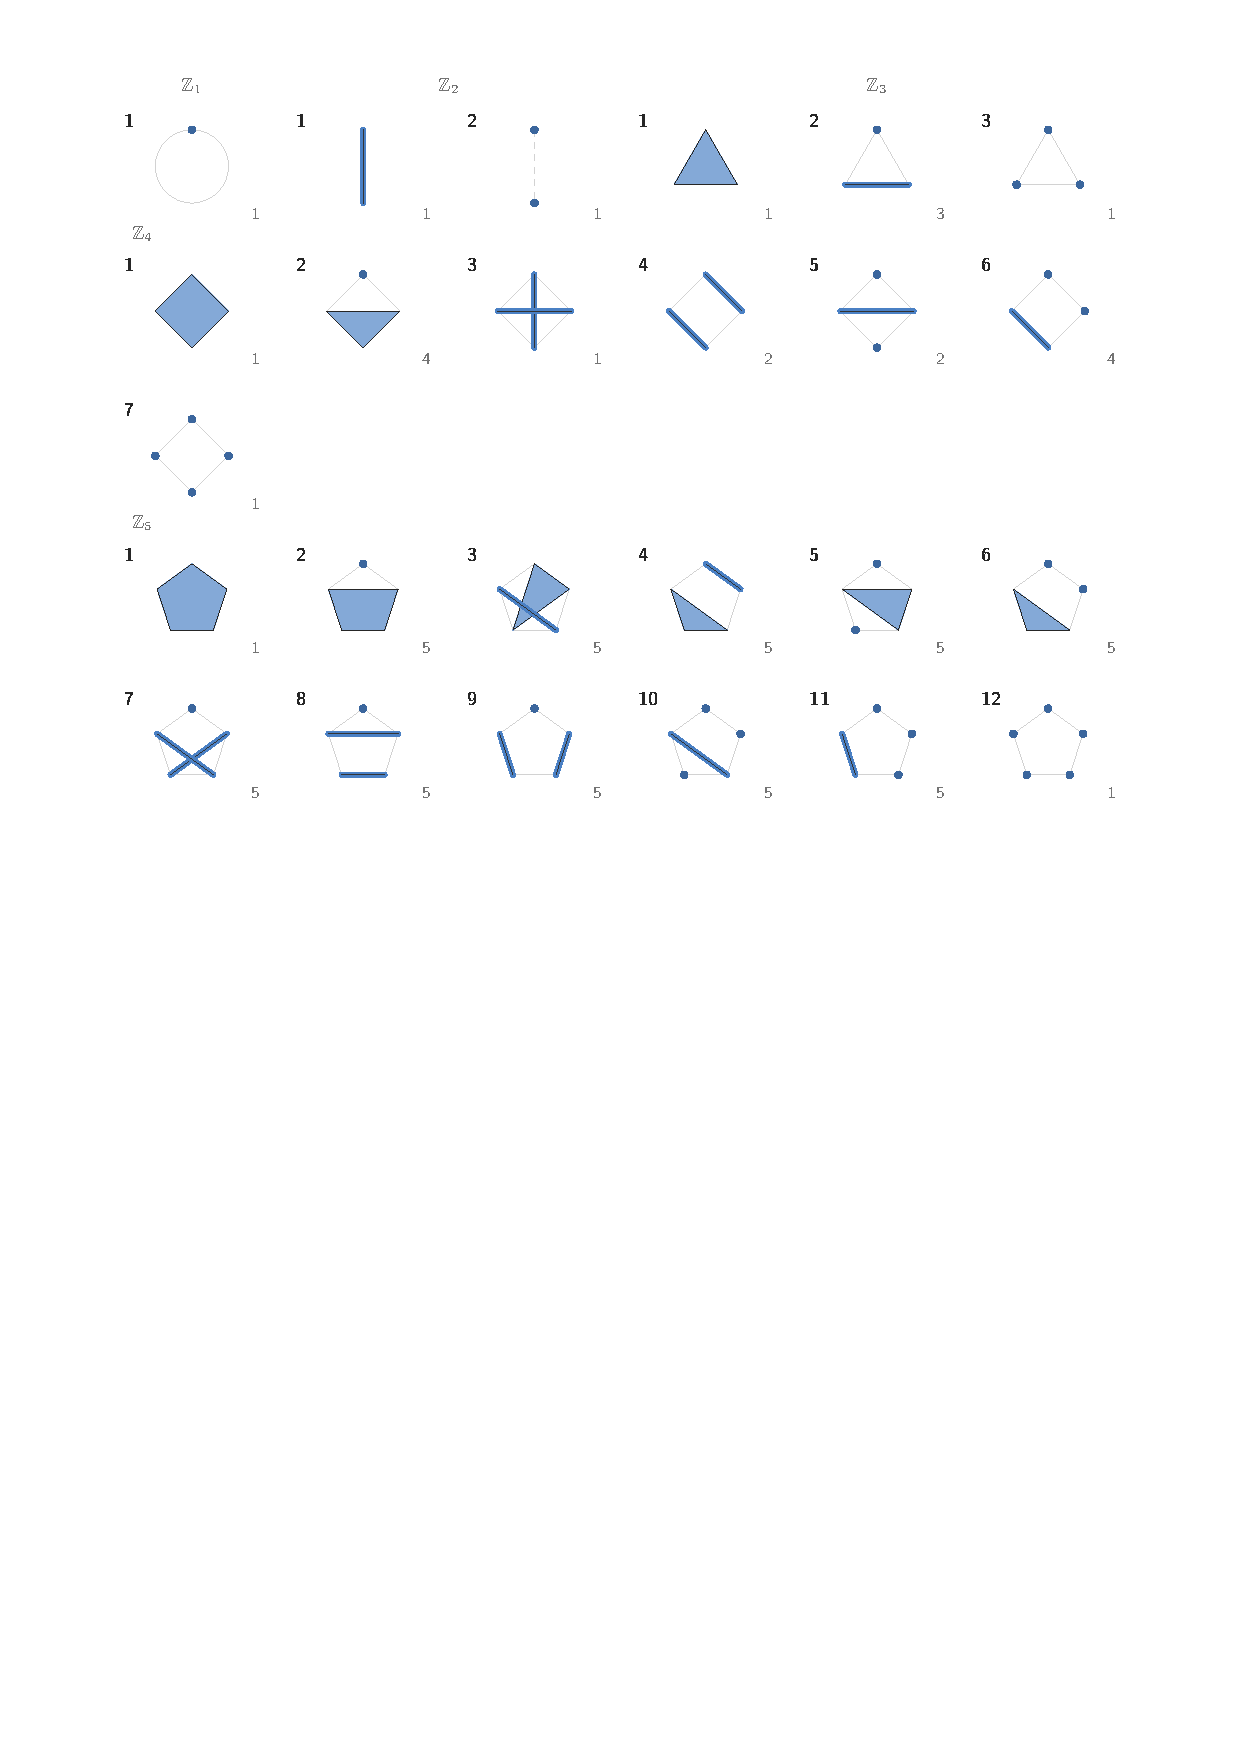
\includepdf[
  pages=-,
  offset=0 -16mm,
  pagecommand={\thispagestyle{headings}},
  addtotoc={
     1, section, 1, {The Small Cyclic Lattices \texorpdfstring{($\mathbb{Z}_1$ through $\mathbb{Z}_5$)}{}}, sec:ring-z1-z5,
     2, section, 1, {The Hexagonal Lattice \texorpdfstring{$\mathbb{Z}_6$}{Z6}}, sec:ring-z6,
     3, section, 1, {The Heptagonal Lattice \texorpdfstring{$\mathbb{Z}_7$}{Z7}}, sec:ring-z7,
     5, section, 1, {The Octagonal Lattice \texorpdfstring{$\mathbb{Z}_8$}{Z8}}, sec:ring-z8
  }
]{plates/plates_z1_z8.pdf}


\backmatter
\chapter*{Suggested Reading}
\addcontentsline{toc}{chapter}{Suggested Reading}
\markboth{Suggested Reading}{Suggested Reading}

This atlas unifies the dihedral geometry of composition mosaics across the elementary cyclic lattices $\mathbb{Z}_1$ through $\mathbb{Z}_8$, bridging integer partitions, circular set partitions, and dihedral equivalence classes. The curated literature below provides foundational theory, classical historical developments, and broader combinatorial and algebraic context.

\section*{Dihedral Enumeration and Orbit Counting}

\begin{description}
    \item[\textbf{Augustin-Louis Cauchy (1845)}]\mbox{}\\
    \emph{M\'emoire sur diverses propri\'et\'es remarquables des substitutions r\'eguli\`eres ou irr\'eguli\`eres, et des syst\`emes de substitutions conjugu\'ees}, \emph{Comptes Rendus de l'Acad\'emie des Sciences}, 21:972--987.\\
    The original formulation of the orbit-counting lemma for permutation groups.

    \item[\textbf{Ferdinand Georg Frobenius (1887)}]\mbox{}\\
    \emph{\"Uber die Congruenz nach einem aus zwei endlichen Gruppen gebildeten Doppelmodul}, \emph{Journal f\"ur die reine und angewandte Mathematik (Crelle's Journal)}, 101:273--299.\\
    The generalisation of the orbit-counting theorem to abstract finite group actions.

    \item[\textbf{William Burnside (1911)}]\mbox{}\\
    \emph{Theory of Groups of Finite Order}, 2nd edition, Cambridge University Press, Cambridge.\\
    The classical treatise popularising the orbit-counting lemma, forming the arithmetic core of dihedral cycle index evaluations on cyclic lattices.

    \item[\textbf{George P\'olya (1937)}]\mbox{}\\
    \emph{Kombinatorische Anzahlbestimmungen f\"ur Gruppen, Graphen und chemische Verbindungen}, \emph{Acta Mathematica}, 68(1):145--254.\\
    The foundational memoir formalising the cycle index polynomial $Z(G; z_1, \dots, z_n)$ and its functional substitution principles for weighted configuration counting under group equivalence.

    \item[\textbf{Harald Fripertinger (1997)}]\mbox{}\\
    \emph{Enumeration of isometry classes of mosaics}, \emph{Discrete Mathematics}, 176(1--3):87--98.\\
    The pioneering combinatorial census of set partitions on cyclic and dihedral lattices, establishing the orbit inventory of geometric mosaics.

    \item[\textbf{Adalbert Kerber (1999)}]\mbox{}\\
    \emph{Applied Finite Group Actions}, 2nd edition, Springer-Verlag, Berlin, Heidelberg.\\
    An exhaustive modern reference on the algebraic apparatus of permutation representations, double-coset decompositions, and constructive orbit generation.
\end{description}

\section*{Set Partitions, Combinatorial Species, and Fa\`a di Bruno Theory}

\begin{description}
    \item[\textbf{Eric Temple Bell (1934)}]\mbox{}\\
    \emph{Exponential polynomials}, \emph{Annals of Mathematics}, 35(2):258--277.\\
    Foundational formulation of exponential polynomials and Bell numbers enumerating set partitions, establishing the combinatorial bedrock of total mosaic volume across $\mathbb{Z}_1 \dots \mathbb{Z}_8$.

    \item[\textbf{Gian-Carlo Rota (1964)}]\mbox{}\\
    \emph{The Number of Partitions of a Set}, \emph{The American Mathematical Monthly}, 71(5):498--504.\\
    The classic modern foundation of partition lattice combinatorics, generating functions, and umbral operator techniques for set partition enumerations.

    \item[\textbf{Andr\'e Joyal (1981)}]\mbox{}\\
    \emph{Une th\'eorie combinatoire des s\'eries formelles}, \emph{Advances in Mathematics}, 42(1):1--82.\\
    The categorical foundation of combinatorial species, providing the functorial machinery underlying Singleton Shattering Duality and cycle index series.

    \item[\textbf{Francesco Fa\`a di Bruno (1855)}]\mbox{}\\
    \emph{Sullo sviluppo delle funzioni}, \emph{Annali di Scienze Matematiche e Fisiche}, 6:479--480.\\
    The classical multinomial expansion governing the derivative of composite functions, structuring the shape-stratified multinomial decomposition of circular compositions.

    \item[\textbf{Philippe Flajolet and Robert Sedgewick (2009)}]\mbox{}\\
    \emph{Analytic Combinatorics}, Cambridge University Press, Cambridge.\\
    The definitive modern treatise on combinatorial constructions, exponential generating functions, and multiset formations under symmetry.
\end{description}

\section*{Difference Systems and Combinatorial Block Designs}

\begin{description}
    \item[\textbf{Thoralf Skolem (1957)}]\mbox{}\\
    \emph{On certain distributions of integers in pairs with given differences}, \emph{Mathematica Scandinavica}, 5:57--68.\\
    The seminal paper introducing difference systems of integer pairs, providing the structural prototype for the unique cyclic Skolem mosaic partition on $\mathbb{Z}_8$.

    \item[\textbf{Duncan M. Y. Sommerville (1909)}]\mbox{}\\
    \emph{On Certain Periodic Properties of Cyclic Compositions of Numbers}, \emph{Proceedings of the London Mathematical Society}, Second Series, 7:263--313.\\
    Early 20th-century foundation for periodic cyclic integer compositions and circular stride geometries.
\end{description}

\section*{The Cyclic Lattice Cartography Trilogy}

\begin{description}
    \item[\textbf{Gemma Knee and Antigra Vitti (2026)}]\mbox{}\\
    \emph{The Polygonal Burnsidean: An Atlas of Inscribed Polygons from $\mathbb{Z}_1$ to $\mathbb{Z}_{16}$}, Newcastle upon Tyne.\\
    The first volume in the trilogy: complete algebraic classification and visual cartography of all 5,099 dihedral orbits of inscribed single polygons across $\mathbb{Z}_1 \dots \mathbb{Z}_{16}$.

    \item[\textbf{Gemma Knee and Antigra Vitti (2026)}]\mbox{}\\
    \emph{Hexadecality: The Atlas of Hexadecagonal Compositions}, Newcastle upon Tyne.\\
    The second volume: exhaustive affine macro-orbit classification and visual plates of the 21,030 macro-orbits (83,488 dihedral comosaics) of uniform tetramers ($z_4^4$) on $\mathbb{Z}_{16}$, alongside the square universes of $\mathbb{Z}_4$ and $\mathbb{Z}_9$.
\end{description}


\end{document}
